\documentclass[a4paper,portuguese,10pt]{article}

\usepackage{setspace}
\usepackage[hang,footnotesize]{caption}
\usepackage[utf8]{inputenc}
\usepackage{graphicx}
%\usepackage{hyperref}
\usepackage[colorlinks=true]{hyperref}
\hypersetup{
  linkcolor=black,
  citecolor=blue,
}
%\usepackage{setspace}
%\usepackage{abntcite}
\usepackage{amsfonts}
\usepackage{amsmath}
\usepackage{nonfloat}
\usepackage{semtrans}
\usepackage[margin=2cm]{geometry}
\usepackage[portuguese]{babel}
\usepackage[fixlanguage]{babelbib}
\selectbiblanguage{portuguese}
\usepackage[svgnames]{xcolor} % Specify colors by their 'svgnames'; list of all colors available: http://www.latextemplates.com/svgnames-colors
\usepackage{titlesec}
\usepackage[numbers]{natbib}
\usepackage{nomencl}
\usepackage{ifthen}
\usepackage{multicol} % use of multiple columns
\usepackage{fancyhdr}
\usepackage{tikz}
\usetikzlibrary{shapes,shadows,arrows}
%\usepackage{draftwatermark}
%\SetWatermarkText{ANNEX 2}
%\SetWatermarkScale{3}
%\SetWatermarkColor[rgb]{red!60}
\columnsep=8mm
%\columnseprule=1pt

\newcommand{\p}{\parallel}
\newcommand{\m}{\mid}
\newcommand{\del}{\bigtriangleup}
\newcommand{\lb}{\linebreak}
\newcommand{\nl}{\newline}
\renewcommand{\div}{{\,\rm div}\,}
\newcommand{\grad}{\,\rm {grad}\,}
\renewcommand{\D}{\partial}
\newcommand{\RR}{\mathbb{R}}
\renewcommand{\vec}{\mathbf}
\newcommand{\esp}{\text{\hspace{2mm}}}
\newcommand{\dgs}{\textordmasculine}
\renewcommand{\max}{\operatorname{max}}
\newcommand{\Ra}{\operatorname{Ra}}
\renewcommand{\Re}{\operatorname{Re}}
\newcommand{\Gr}{\operatorname{Gr}}
\newcommand{\St}{\operatorname{St}}
\renewcommand{\Pr}{\operatorname{Pr}}
\newcommand{\CFL}{\operatorname{CFL}}

%\setlength{\hoffset}{-1cm}
%\setlength{\textwidth}{17cm}
%\setlength{\parskip}{1cm plus4mm minus3mm}
\setlength{\parskip}{2mm}
\setlength{\parindent}{0mm} % Default is 15pt.
\titleformat*{\section}{\normalsize\bfseries}
\titleformat*{\subsection}{\normalsize\bfseries}

\renewcommand{\refname}{\normalsize{References}}
\renewcommand{\nomname}{List of Symbols}

\renewcommand{\nomgroup}[1]{%
\ifthenelse{\equal{#1}{R}}{\item[\textbf{Roman letters}]}{%
\ifthenelse{\equal{#1}{G}}{\item[Greek letters]}{}}}

\pagestyle{fancy}
\lhead{}
\rhead{\small{Sistemas Passivos de Resfriamento}}


%%%%%%%%%%%%%%%%%%%%%%%%%%%%%%%%%%%%%%%%%%%%%%%%%%%%%%%%%%%%%%%%%%%%%%%%%%%%%%%%%%
\begin{document}

\thispagestyle{empty}

\begin{minipage}{0.5\linewidth}
\large\textbf{RELATÓRIO\\TÉCNICO}
\end{minipage}
\begin{minipage}{0.5\linewidth}
\flushright
%\includegraphics[height=2cm]{../../imagens/logoeletronuclear.jpg}
%\includegraphics[height=18mm]{../../imagens/logouerj.jpg}
%\hspace{.5cm}
%\includegraphics[height=15mm]{../imagens/logo_tu_dresden.png}\\
\end{minipage}

\hrulefill

%\begin{minipage}[b]{0.5\linewidth}
\Large \color{NavyBlue} \textbf{SISTEMAS PASSIVOS DE RESFRIAMENTO}\\
\color{Black}\\ % Title
%\vspace{-.5cm}
\normalsize \texttt{Preparado por: Leon Lima}\\%[0.5cm] % Author(s)
\normalsize \texttt{\today}
%\end{minipage}

%\begin{minipage}[b]{0.5\linewidth}
%\flushright
%\includegraphics[height=2cm]{../../imagens/logoeletronuclear.jpg}
%\hspace{.5cm}
%\includegraphics[height=2cm]{../../imagens/logouerj.jpg}\\
%\end{minipage}

\vspace{-2mm}
\hrulefill
\begin{center}
\begin{minipage}{0.8\linewidth}
\footnotesize{\textbf{Resumo.} Este texto busca apresentar as principais características de um Sistema Passivo de Resfriamento, com ênfase na estabilidade termo-hidráulica, abordando os tipos de instabilidades que podem ocorrer em tais sistemas bem como os métodos de análise. A abordagem é feita levando em conta tanto sistemas monofásicos quanto bifásicos. Ênfase, no entanto, é dada a sistemas monofásicos. Sistemas operando em condições supercríticas também são mencionados. Os fatores que influenciam na capacidade de transferência de calor e na estabilidade de tais sistemas são apresentados. Apesar da aplicação de sistemas passivos de resfriamento ser ampla, este texto considera principalmente seu papel em instalações nucleares.}
\end{minipage}
\end{center}
\hrulefill

%\begin{multicols}{2}


\tableofcontents
\hrulefill\\
\onehalfspacing
\section{Introdução}

Sistemas Passivos de Resfriamento (SPRs) consistem essencialmente de circuitos hidráulicos conectados a trocadores de calor que realizam a função de troca térmica sem o auxílio de equipamentos ativos (equipamentos movidos a fontes externas de energia), tais como bombas e ventiladores. As grandes duas vantagens de SPRs são, portanto, a eliminação do custo com fornecimento de energia e o maior grau de confiabilidade do sistema, já que não está sujeito a eventuais interrupções no suprimento de energia e nem a falhas de componentes ativos. Tais vantagens fazem com que SPRs sejam largamente empregados em diversas áreas de engenharia. As primeiras aplicações em grande escala de SPRs ocorreram na indústria automobilística, no resfriamento do bloco de motores de automóveis \cite{VIJAYAN05a}. Realmente, e apesar de \citet{VIJAYAN05a} afirmarem que tal aplicação tenha sido interrompida no final dos anos 1940 com o advento de motores de combustão a altas razões de compressão, o DKW-Vemag, fig.\ref{fig_DKW}, modelo fabricado de 1958 a 1967 no Brasil, usava um circuito a convecção natural no sistema de resfriamento do motor, sendo um dos aspectos que conferiam alta durabilidade a este automóvel. Hoje em dia, sistemas passivos encontram muita aplicação no resfriamento de componentes eletrônicos e na indústria nuclear. De fato, o maior grau de confiabilidade faz com que tais sistemas sejam particularmente relevantes em instalações nucleares, especialmente após os eventos de Fukushima\footnote{Acidente nuclear provocado por forte abalo sísmico sucedido de tsunami que assolou a costa leste do Japão. O tsunami inundou a central nuclear de Fukushima Daiichi, levando os geradores diesel de emergência a falha. O corte da energia suprida pelos geradores diesel ocasionou a perda da capacidade de resfriamento dos reatores e culminou com o derretimento do núcleo de pelo menos uma das unidades da central.}.

\begin{center}
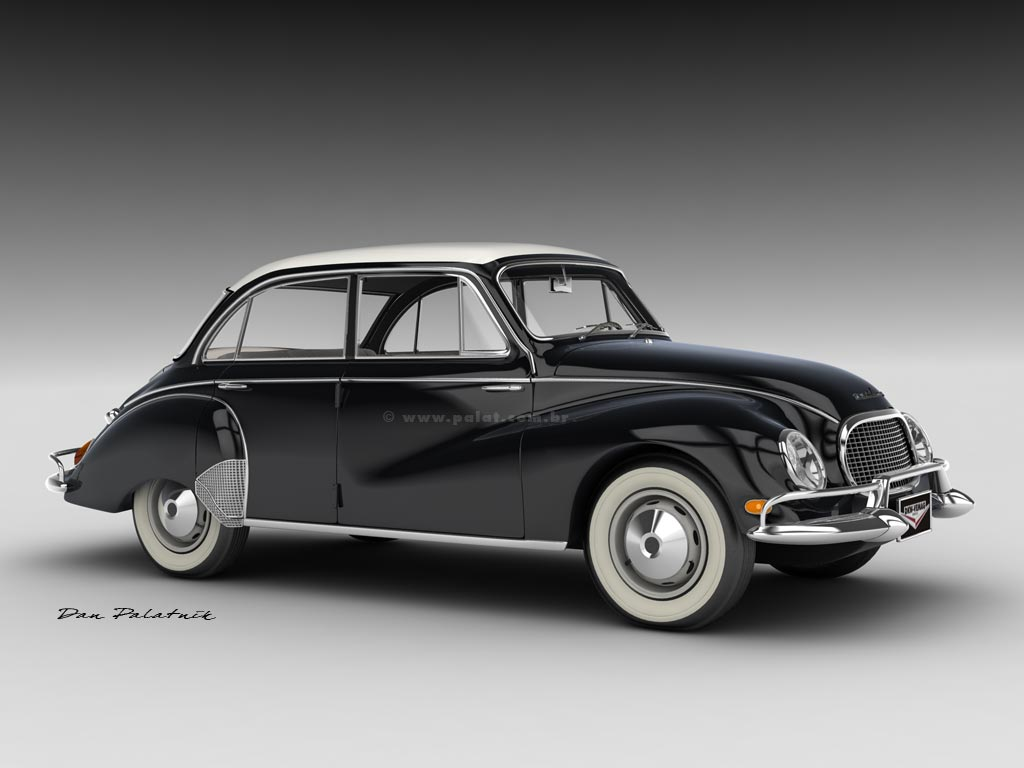
\includegraphics[width=.4\columnwidth]{../imagens/jpg/DKW-Vemag_Belcar.jpg}
\figcaption{DKW-Vemag Belcar. Este automóvel foi fabricado no Brasil entre 1958 e 1967 pela Vemag, sob licença da montadora alemã DKW (sigla para Dampf Kraft Wagen, que significa ``Carro de Força a Vapor'').}
\label{fig_DKW}
\end{center}

A força motriz de um SPR é o empuxo gerado ou pela distribuição não uniforme de temperatura ou por mudança de fase ao longo do circuito. Em regime permanente (equilíbrio), a soma das forças de empuxo do circuito é igual à soma das forças de arrasto. SPRs operam, portanto, por convecção natural e podem ser monofásicos ou bifásicos. Sistemas monofásicos operam com cargas térmicas bem menores em relação a sistemas bifásicos, porém necessitam de menores dimensões verticais, tornando interessante sua aplicação em resfriamento de palhetas de turbinas a gás, aquecedores solares e refrigeradores \cite{BASU13b}.

Há sistemas monofásicos capazes de transferir cargas térmicas mais altas. São aqueles que operam em condições termodinâmicas supercríticas, isto é, acima do ponto crítico termodinâmico. Apesar de serem classificados como monofásicos, esses sistemas podem apresentar características tanto de líquido quanto de gás. Por operarem a altas temperaturas, são muito empregados em ciclos térmicos para geração de energia. Muitas usinas termoelétricas a combustíveis fósseis utilizam água supercrítica em razão do elevado rendimento térmico: enquanto ciclos convencionais podem apresentar rendimentos de até 36\%, ciclos supercríticos podem chegar a 50\% de rendimento \cite{SCHULENBERG14}. Além disso, sua aplicação em sistemas passivos é favorecida pelos altos gradientes de densidade próximos de pontos pseudo-críticos\footnote{Para cada curva isobárica acima da pressão crítica, existe uma temperatura supercrítica que define um ponto pseudo-crítico nessa isobárica, no qual o calor específico a pressão constante exibe um valor máximo.}. Um dos projetos da Geração IV de reatores nucleares\footnote{\href{https://www.gen-4.org/gif/jcms/c_9260/public}{www.gen-4.org}} \cite{GOLDBERG11} consiste num reator resfriado a água supercrítica, possivelmente com sistemas passivos \cite{OKA95,BUONGIORNO03,SCHULENBERG11}.

No entanto, sejam monofásicos ou bifásicos, SPRs possuem a desvantagem de estarem sujeitos a instabilidades, o que pode provocar vibrações indesejáveis no circuito e prejudicar a função de remoção de calor localmente, gerando pontos com picos de temperatura. Apesar de sistemas bifásicos serem bem mais suscetíveis a esse problema, há condições nas quais sistemas monofásicos também podem ser instáveis.

As próximas seções buscam aprofundar os aspectos principais relacionados a SPRs. A seção \ref{sec_projeto} sumariza os parâmetros de projeto mais relevantes que devem ser levados em conta no desenvolvimento de um SPR. Na seção \ref{sec_estabilidade}, uma classificação dos tipos de estabilidade é apresentada, baseada em referências clássicas adotadas nesta área. Uma modelagem matemática para sistemas monofásicos (convencionais) é descrita na seção \ref{sec_modelo}, e resultados de validação do modelo são apresentados na mesma seção. A última seção apresenta uma descrição breve do sistema passivo de resfriamento da Unidade UFC, que é a instalação destinada a armazenar os Elementos Combustíveis Irradiados na CNAAA, sendo projetada pela Eletrobras Eletronuclear.

\section{Projeto de Sistema Passivo de Resfriamento\label{sec_projeto}}

A finalidade de um sistema de resfriamento é manter a temperatura de algum componente, ambiente ou sistema abaixo de um limite de projeto. Para isso ele deve transferir calor da fonte quente (que é o componente, ambiente ou sistema) para uma fonte fria. Em muitos casos, a fonte quente não está próxima da fonte fria, e o sistema de resfriamento deve conduzir o calor através de um circuito. Portanto, a composição básica de um Sistema Passivo de Resfriamento consiste de um circuito hidráulico (termicamente isolado) que conecta um trocador que absorve calor da fonte quente a outro trocador que rejeita o calor à fonte fria. 

Se conectarmos um circuito qualquer com esses componentes a uma fonte quente e uma fonte fria, o circuito certamente transferirá o calor gerado pela fonte quente. O ponto relevante é a que diferença de temperatura ele realiza esse transporte. Num sistema forçado, é mais fácil ajustar uma vazão tal que o calor seja transferido a uma diferença de temperatura adequada. Para sistemas de convecção natural, esse ajuste deve ser feito no projeto do circuito, de maneira a proporcionar uma vazão igual ou superior a um limite que garanta uma diferença de temperatura abaixo dos limites de projeto. Para tanto, é necessário levar em conta o balanço entre as forças de empuxo e as forças de arrasto atuantes, em função do qual a velocidade de escoamento que vai equilibrar essas forças é determinada. No projeto do sistema, a velocidade que fecha o balanço é obtida através do ajuste de duas variáveis independentes. A primeira é a ``altura'' do circuito, ou melhor, a diferença de nível entre os trocadores de calor. Quanto maior esta diferença, maior será o empuxo gerado, proporcionando maiores vazões. A segunda variável são as perdas de carga no circuito, que são função de parâmetros geométricos como diâmetro interno, comprimentos e perdas localizadas. Através dessas duas variáveis de projeto, o circuito pode ser dimensionado de forma a proporcionar a vazão adequada para a diferença de temperatura limite.

É preciso notar, contudo, que o dimensionamento do circuito depende também da eficiência dos trocadores de calor. Trocadores com baixa eficiência requerem maiores diferenças entre lado quente e lado frio para a troca, o que reduz o $\Delta T$ no circuito, exigindo, por fim, maior vazão para que o limite de temperatura projetado não seja ultrapassado. O {\it design} de um trocador de calor eficiente é, talvez, o ponto mais complexo no projeto de um SPR, porque envolve convecção térmica em geometrias complexas, em regimes muitas vezes turbulento, e exige conhecimento da condutividade térmica do material.

\subsection{Estabilidade {\it vs} vazão}

Existe ainda um outro fator que deve ser considerado no projeto de um SPR: a estabilidade termo-hidráulica do sistema. A interação livre entre forças de empuxo e de arrasto pode levar um SPR a comportamentos instáveis, e a relação entre empuxo e arrasto ajustada para proporcionar uma vazão maior pode ser favorável ao surgimento de instabilidades, já que as perdas por atrito ao longo do circuito tendem a estabilizar o sistema. Outros fatores como a direção e sentido do escoamento pelos trocadores de calor e eventuais inclinações do circuito também exercem influência sobre a estabilidade termo-hidráulica de um SPR. Neste contexto, a escolha correta de parâmetros geométricos como diâmetro interno, altura e comprimento do circuito é fundamental. Quanto menor o diâmetro interno, mais estável tende a ser o sistema, porém a vazão reduz sensivelmente. Segundo \citet{BASU13b}, aumentar a altura do circuito é uma opção melhor pois tende a estabilizar o sistema proporcionando vazões maiores.

O efeito do diâmetro no estado permanente e na estabilidade de sistemas monofásicos e bifásicos também foi estudado por \citet{VIJAYAN08}, os quais também concluem que o aumento do diâmetro é favorável para a vazão no circuito mas tende a desestabilizar o escoamento. A estabilidade termo-hidráulica de um SPR também é influenciada pela carga térmica, tanto pelo valor instantâneo quanto pelo gradiente. Esse efeito foi estudado por \citet{BASU13a}. Outro parâmetro relevante é a orientação dos trocadores de calor (fluxo predominantemente horizontal ou vertical), conforme estudado por \citet{VIJAYAN07}. O volume dos trocadores de calor também pode contribuir para estabilizar o escoamento, conforme concluem \citet{TJOEN12}. Um estudo comparativo entre sistemas monofásicos, bifásicos e supercríticos foi realizado por \citet{VIJAYAN10}, levando em conta os efeitos de diferentes diâmetros e cargas térmicas no estado permanente do sistema e na estabilidade. Seus resultados são reproduzidos aqui nas figuras \ref{fig_sist_monofasico}, \ref{fig_sist_bifasico} e \ref{fig_sist_supercritico} e ilustram bem a influência do diâmetro e da carga térmica na vazão e na estabilidade dos sistemas. As figuras mostram a variação da vazão em função da carga térmica e mapas de estabilidade para três diâmetros diferentes. O mapa de estabilidade para sistemas monofásicos (fig. \ref{fig_sist_monofasico}) é apresentado em função dos números de Stanton (St) e de Grashof (Gr) modificados \cite{VIJAYAN94}, sendo St mais associado ao coeficiente de troca térmica do arrefecedor e Gr mais associado à carga térmica.

\begin{figure}
  \begin{center}
    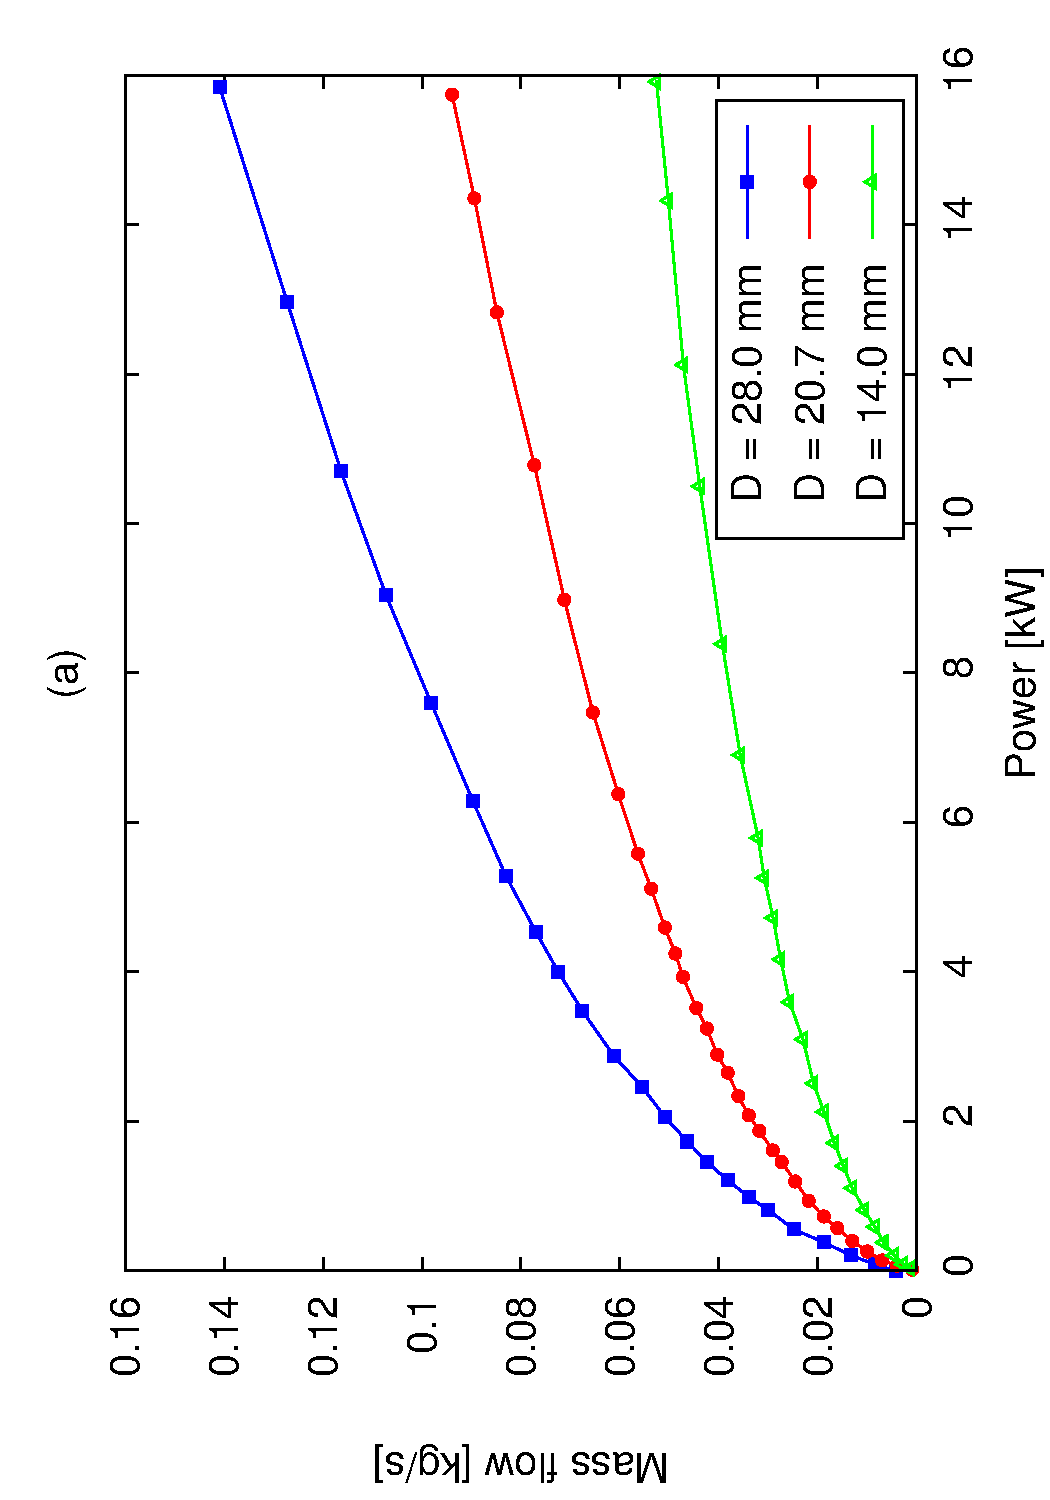
\includegraphics[width=.3\linewidth,angle=-90,origin=c]{../imagens/pdf/mxQ_sp.pdf}
    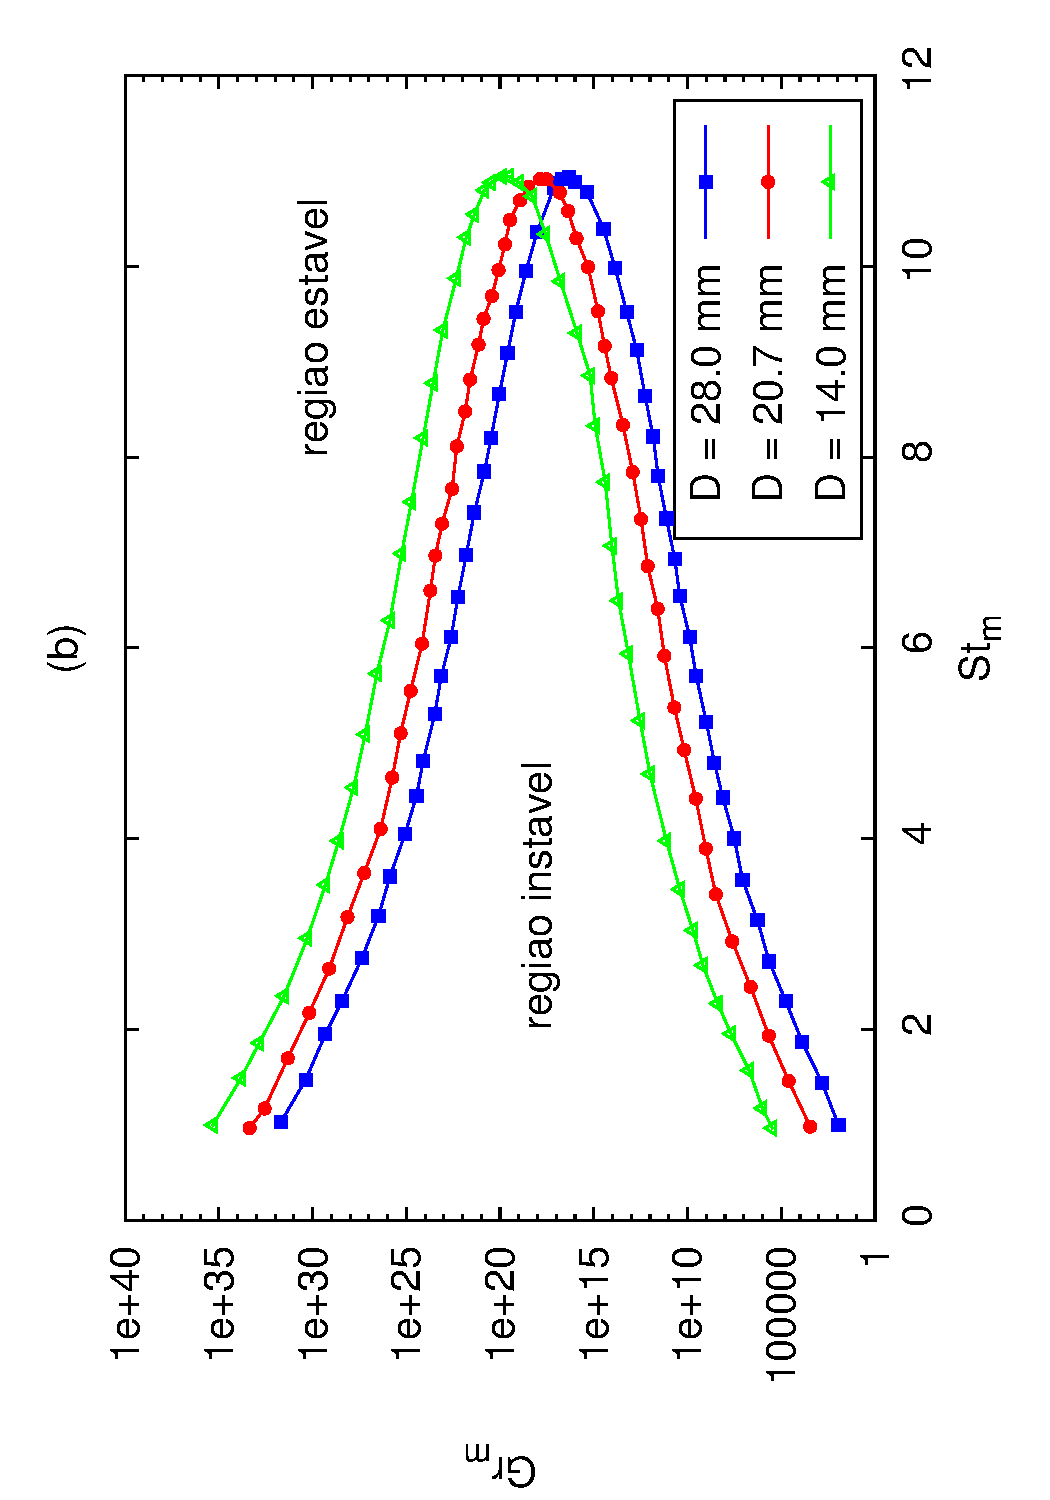
\includegraphics[width=.3\linewidth,angle=-90,origin=c]{../imagens/pdf/estab_sp.pdf}
    \vspace*{-10mm}
    \figcaption{Sistema monofásico: (a) vazão mássica em função da carga térmica e (b) mapa de estabilidade para três diâmetros diferentes.}
    \label{fig_sist_monofasico}
  \end{center}
\end{figure}

\begin{figure}
  \begin{center}
    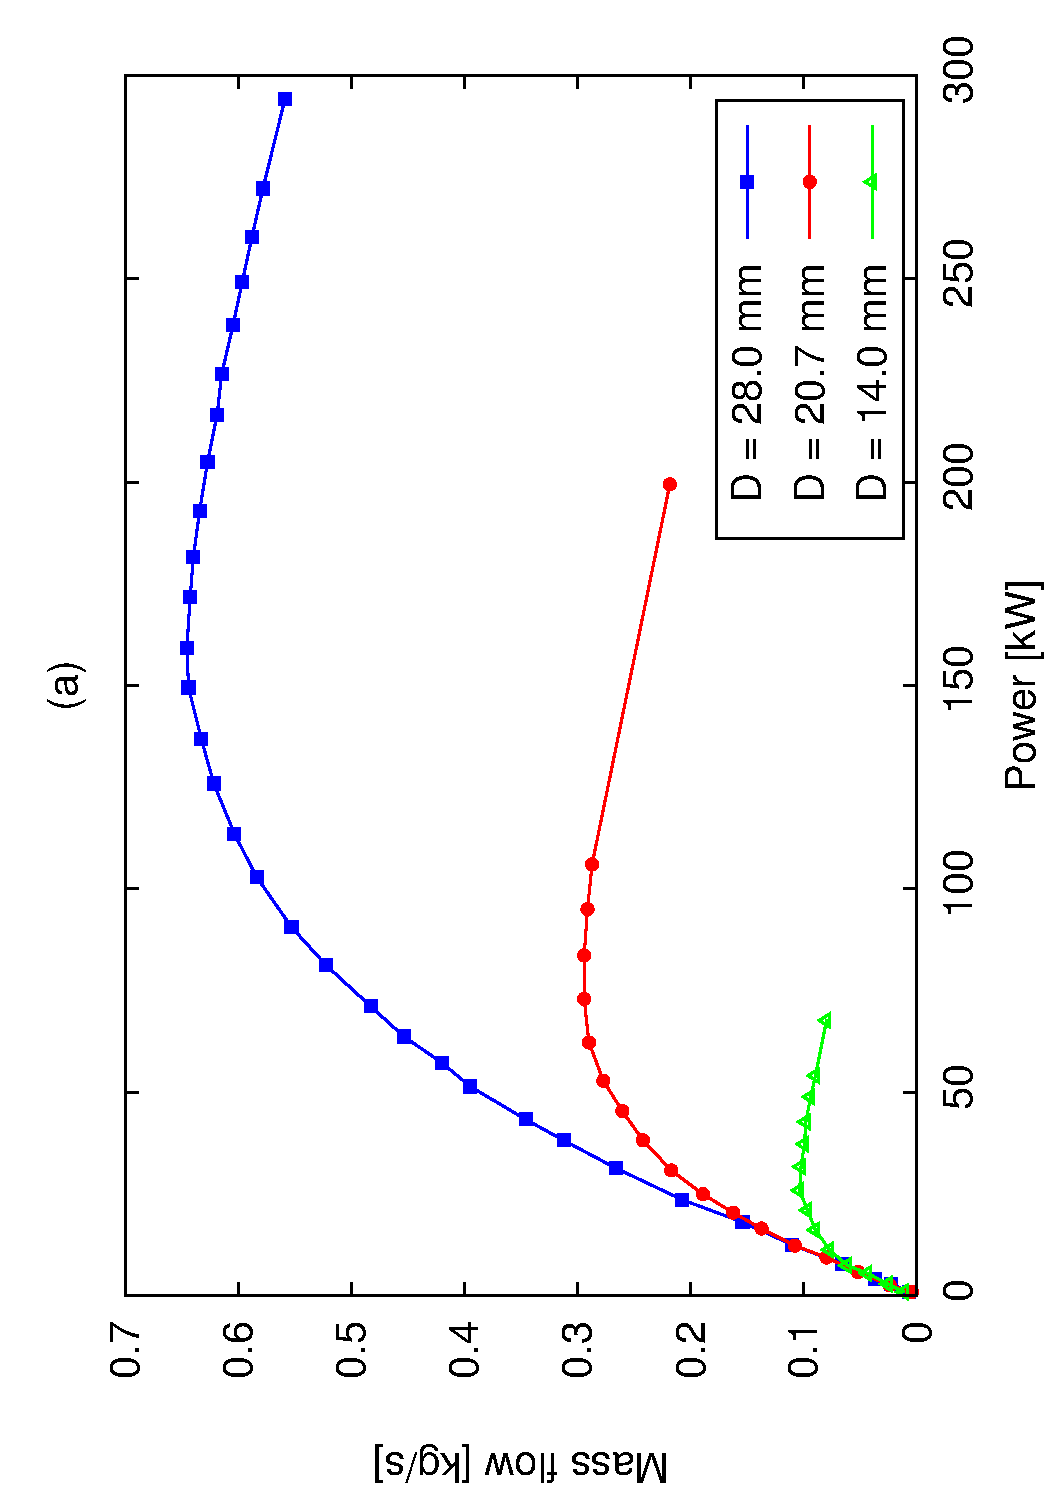
\includegraphics[width=.3\linewidth,angle=-90,origin=c]{../imagens/pdf/mxQ_tp.pdf}
    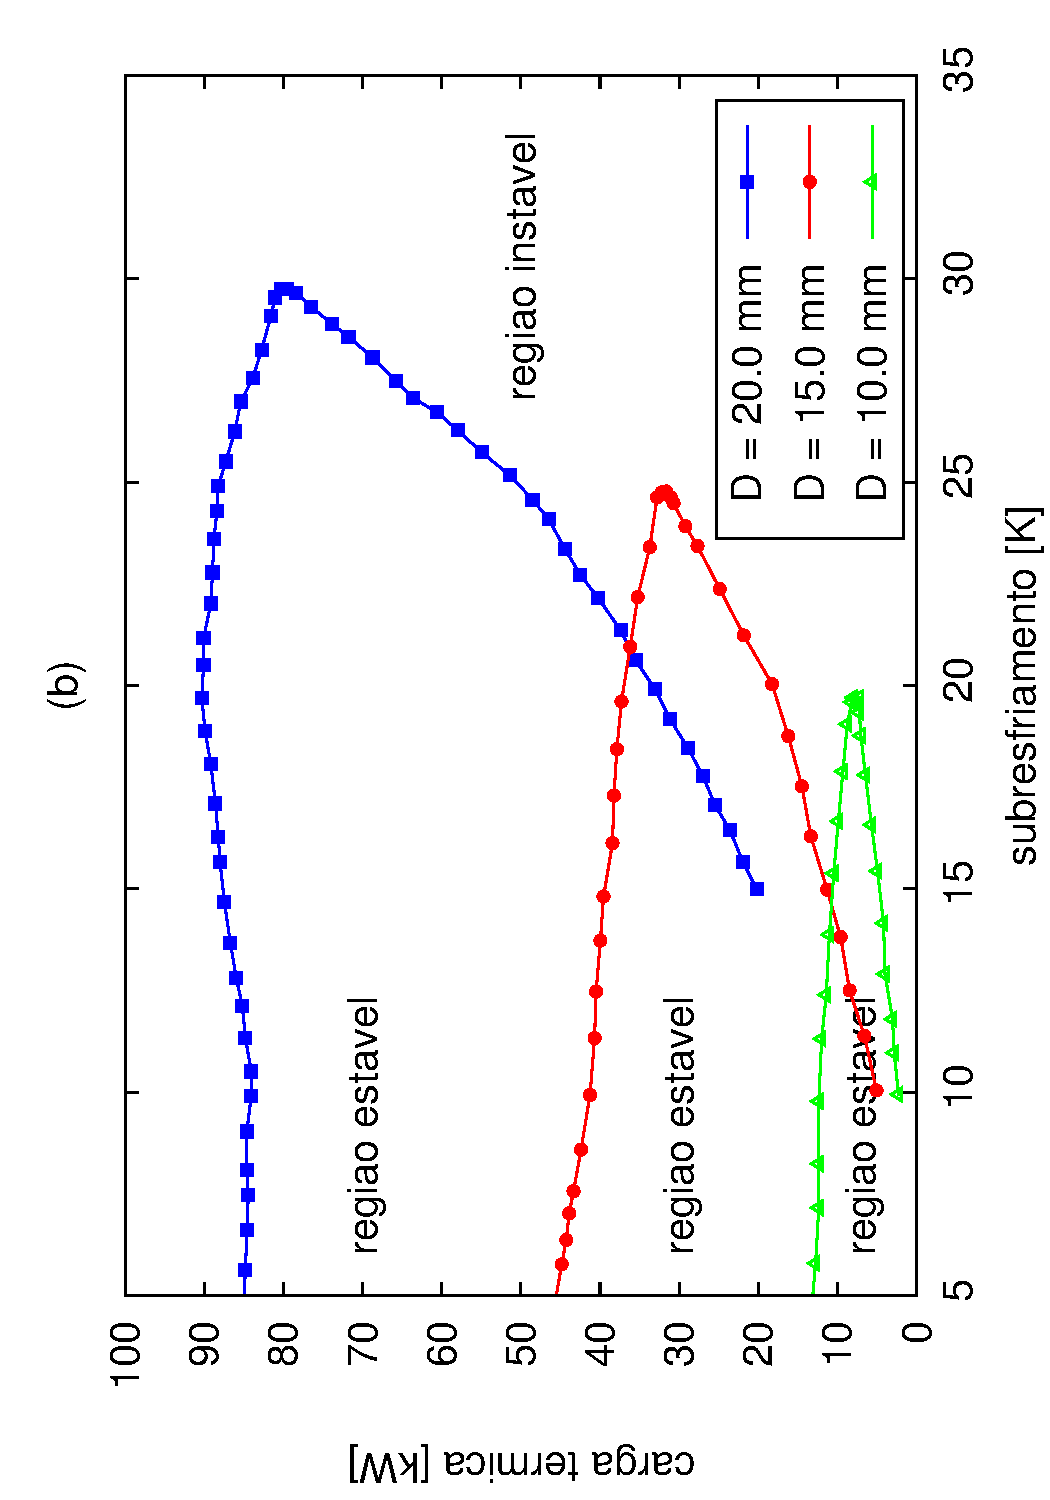
\includegraphics[width=.3\linewidth,angle=-90,origin=c]{../imagens/pdf/estab_tp.pdf}
    \vspace*{-10mm}
    \figcaption{Sistema bifásico: (a) vazão mássica em função da carga térmica e (b) mapa de estabilidade para três diâmetros diferentes.}
    \label{fig_sist_bifasico}
  \end{center}
\end{figure}

\begin{figure}
  \begin{center}
    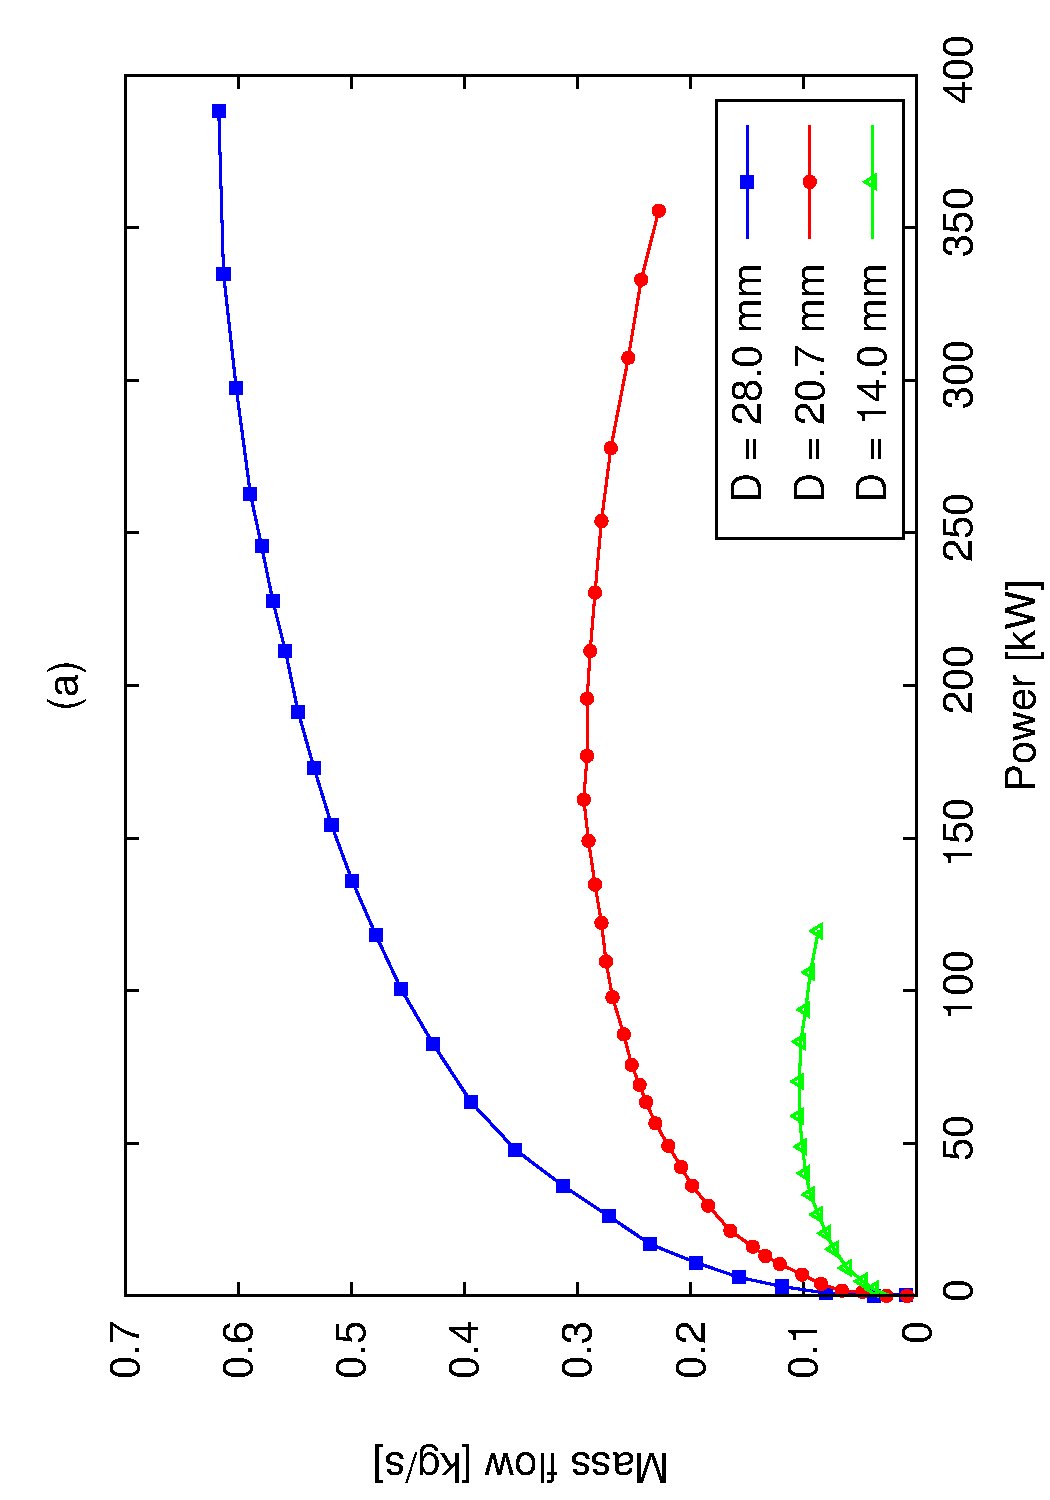
\includegraphics[width=.3\linewidth,angle=-90,origin=c]{../imagens/pdf/mxQ_sc.pdf}
    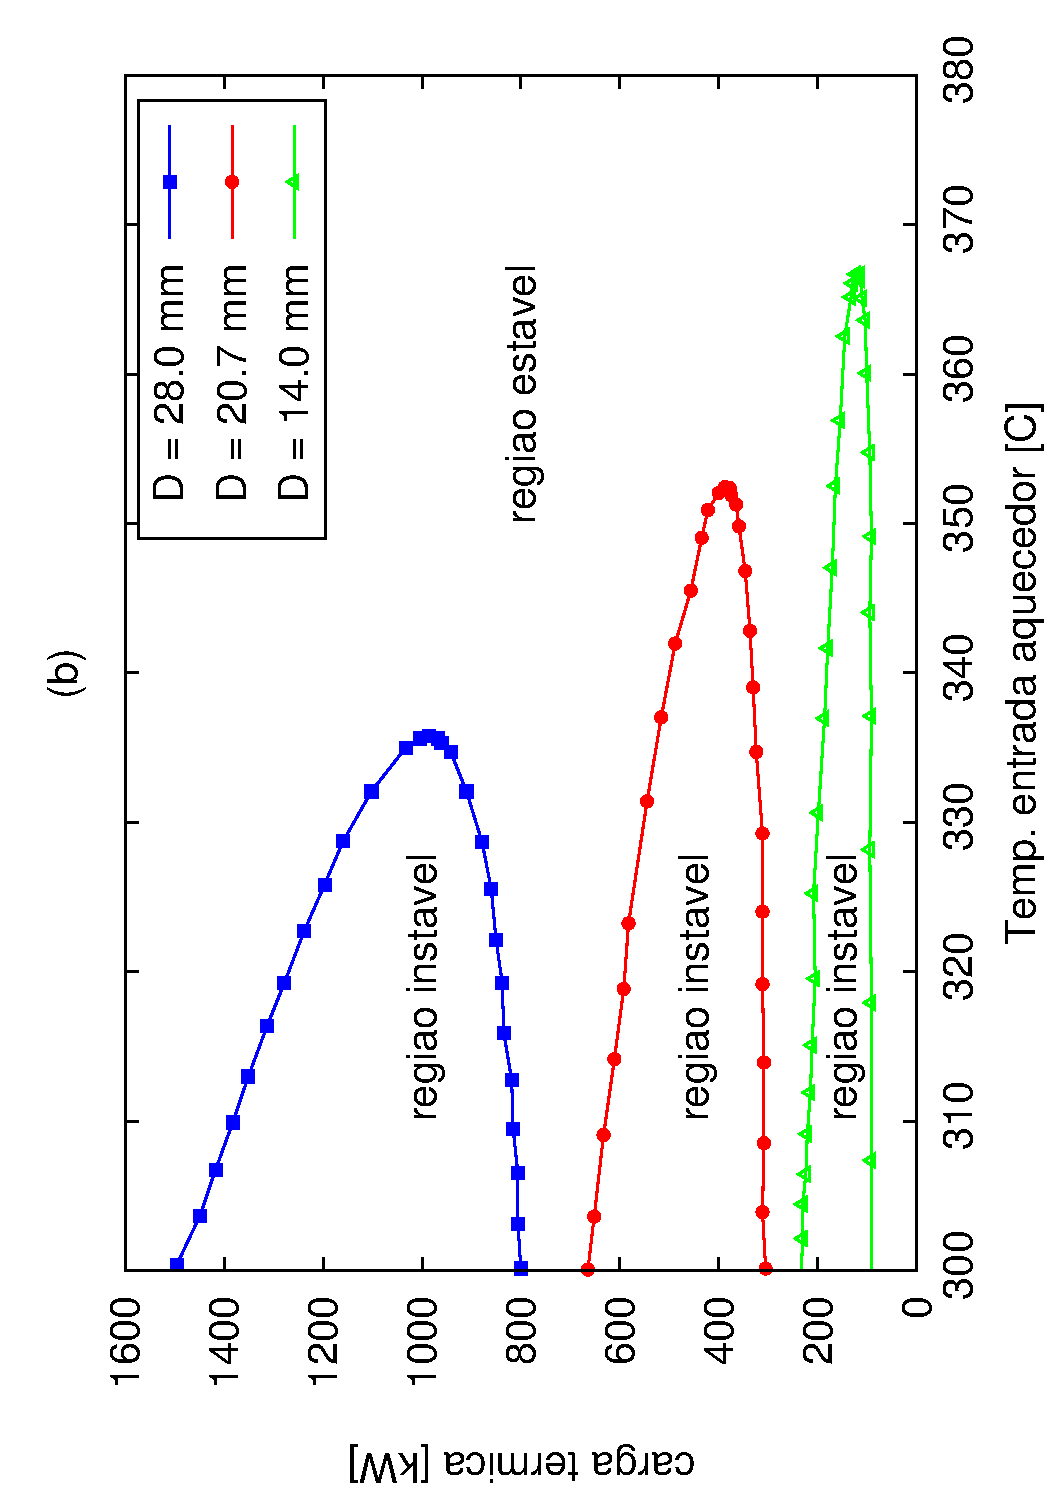
\includegraphics[width=.3\linewidth,angle=-90,origin=c]{../imagens/pdf/estab_sc.pdf}
    \vspace*{-10mm}
    \figcaption{Sistema supercrítico: (a) vazão mássica em função da carga térmica e (b) mapa de estabilidade para três diâmetros diferentes.}
    \label{fig_sist_supercritico}
  \end{center}
\end{figure}

Para sistemas monofásicos, a vazão aumenta monotonicamente com o aumento da carga térmica. Quanto à estabilidade, o aumento do diâmetro desloca a região de instabilidade para baixo no gráfico da figura \ref{fig_sist_monofasico}(b), ou seja, para regiões que provavelmente abrangem condições operacionais mais usuais.

Para sistemas bifásicos, a vazão aumenta com a carga térmica até um certo limite, após o qual ela passa a decrescer com o aumento da carga térmica. A estabilidade do escoamento apresenta respostas totalmente diferentes em relação a sistemas monofásicos, com o aumento do diâmetro gerando regiões de estabilidade maiores. Conforme a figura \ref{fig_sist_bifasico}, as regiões de estabilidade são aquelas ``cercadas'' pelas linhas neutras (ao contrário do que ocorre em sistemas monofásicos e supercríticos). Essa inversão é um indício da existência de regiões com naturezas distintas de instabilidade, conforme será abordado em mais detalhes na seção \ref{sec_estabilidade}.

Para sistemas supercríticos, o comportamento quanto à vazão é parecido com o de sistemas bifásicos, onde, para um dado diâmetro, há um limite após a qual a vazão decresce com o aumento da carga térmica. O comportamento quanto à estabilidade, no entanto, é análogo ao de sistemas monofásicos, com a região instável ``cercada'' pela linha neutra. Para a faixa operacional mostrada na figura \ref{fig_sist_supercritico}, diâmetros maiores deslocam a área de instabilidade para cima no gráfico.

A interação entre aumento de vazão e estabilidade termo-hidráulica do sistema, portanto, deve ser levada em conta no projeto de SPRs.

\subsection{Condição termodinâmica}

O projeto de um SPR também inclui a escolha do tipo de sistema quanto a mudança de fase, já que sistemas monofásicos possuem um limite em relação à carga térmica máxima que podem transferir. Conforme mencionado por \citet{FUCHS13}, a eficiência de troca térmica em sistemas bifásicos é algumas ordens de grandeza superior àquela de sistemas monofásicos, assim como o empuxo disponível. O mesmo ocorre em sistemas que operam acima do ponto crítico termodinâmico (supercríticos). Contudo, SPRs bifásicos e supercríticos, além de envolverem materiais mais sofisticados, são muito mais suscetíveis à instabilidades, conforme será visto na seção \ref{sec_estabilidade}, de maneira que análises de estabilidade são uma etapa importante no projeto de tais sistemas.

Sistemas operando em condições supercríticas são empregados há décadas em usinas termoelétricas a combustíveis fósseis (neste caso, com circulação forçada). Mas a possibilidade de aplicar SPRs em condições supercríticas na indústria nuclear ganhou muita importância com o conceito de reator resfriado a água supercrítica, que é um dos {\it designs} que compõem a chamada Geração IV de reatores nucleares. Conforme já mencionado aqui, o ciclo térmico operando em condições supercríticas pode oferecer eficiências de até 50\%, e os altos gradientes de densidade inerentes a sistemas nessas condições favorece a utilização de circulação passiva. \citet{SARKAR14} explicam que sistemas supercríticos integram vantagens dos circuitos monofásicos, como a alta capacidade de transferência de calor por condução, com vantagens de circuitos bifásicos, como as altas vazões sem separação de fases. Muitos trabalhos recentes têm se dedicado a SPR em condições supercríticas. Como referência, vale citar as revisões de \citet{SARKAR14} e \citet{SCHULENBERG14}.

\section{Estabilidade\label{sec_estabilidade}}

O conceito físico de estabilidade é bastante intuitivo, porque está presente no dia-a-dia de qualquer pessoa. É comum, por exemplo, após posicionar um objeto num local um pouco mais delicado, alguém dar uma ``pequena empurrada'' para observar se o posicionamento será mantido. Este procedimento, na verdade, constitui uma análise de estabilidade do estado permanente daquele objeto, ou seja, a partir da introdução de uma pequena perturbação (empurrada) no estado permanente do objeto, observar se ele retorna à configuração inicial (se retornar então o posicionamento é estável para aquela amplitude de perturbação).

A partir deste conceito, é possível estabelecer uma definição geral para estabilidade. Se um sistema, após submetido a uma perturbação, retorna a seu estado permanente original, então ele é estável. Caso contrário, ele é instável. Muitos autores consideram ainda uma terceira condição, dita neutralmente estável, na qual o sistema, após uma perturbação, passa a oscilar com uma amplitude constante.

Do ponto de vista matemático, instabilidades em SPRs estão associadas a múltiplas soluções para os balanços de massa, energia e quantidade de movimento no circuito, numa condição tal que o sistema não converge para uma delas. Conforme explicado por \citet{VIJAYAN05b}, o comportamento instável surge quando o sistema, ao se aproximar de uma solução permanente, gera uma resposta que faz com que outra solução se torne mais atraente, levando o sistema a buscar essa nova solução. O ciclo prossegue com a geração de uma nova resposta de sinal oposto, mantendo o comportamento oscilatório do sistema.

\subsection{Diferenças entre sistemas monofásicos e bifásicos quanto à estabilidade}

Comportamentos instáveis são mais bem mais comuns em sistemas bifásicos. Conforme será apresentado na seção \ref{sec_tipos}, instabilidades podem ser classificadas em diversos tipos, e todos eles podem ocorrer em sistemas bifásicos, mas nem todos ocorrem em sistemas monofásicos.

De fato, \citet{CREVELING75}, em artigo científico de 1975, relatam que instabilidades em SPR monofásicos haviam sido, até então, relatadas apenas para sistemas operando em condições próximas ao ponto crítico termodinâmico. Os comportamentos instáveis observados nesses trabalhos foram associados às fortes variações das propriedades termodinâmicas em condições próximas às do ponto crítico. \citet{CREVELING75} citam, contudo, resultados analíticos publicados entre 1966 e 1967 que concluíram haver condições nas quais SPRs operando com fluido em condições convencionais (subcríticas) apresentam instabilidades. Motivado pela evidência analítica, \citet{CREVELING75} foi o primeiro trabalho a demonstrar experimentalmente a ocorrência de instabilidades num circuito de convecção natural em condições convencionais.

Hoje existe conhecimento amplo a respeito das instabilidades que podem ocorrer em sistemas monofásicos de convecção natural. Em particular, muitos estudos foram realizados pelo Centro de Pesquisa Atômica de Bhabha, em Mumbai, na Índia \cite{VIJAYAN94,NAYAK95,VIJAYAN07,VIJAYAN08,VIJAYAN10}. \citet{VIJAYAN07} afirmam, por exemplo, que a estabilidade de um SPR monofásico depende 

\begin{itemize}
\item dos números de Grashof e Stanton\footnote{Estes adimensionais são apresentados numa forma modificada \cite{VIJAYAN07}.};
\item da razão entre comprimento e diâmetro do circuito;
\item do regime do escoamento;
\item da orientação do aquecedor e resfriador;
\item da direção do escoamento (se ascendente ou descendente no aquecedor e resfriador, caso sejam verticais);
\item e das escalas de comprimento (altura do circuito, comprimento total, comprimento do aquecedor etc.).
\end{itemize}

Diversos resultados experimentais e numéricos em diversas geometrias reproduzem instabilidades, tanto estáticas quanto dinâmicas (ver seção \ref{sec_tipos}), em circuitos de convecção natural monofásicos em condições subcríticas. Escoamentos por convecção natural sem mudança de fase em circuitos fechados ocorrem em vários tipos de instalações nucleares, sendo observados na maioria dos reatores pressurizados em casos de perda das bombas de resfriamento do reator, além de ser a forma de escoamento durante a partida em reatores de água fervente \cite{VIJAYAN05b}.

\subsection{Tipos de instabilidade\label{sec_tipos}}

Os comportamentos quanto à estabilidade de um SPR podem ser classificados em diversos tipos. \citet{BOURE73} foram os primeiros a apresentar uma classificação dos tipos de instabilidade em circuitos resfriamento (incluindo sistemas ativos), em 1973. Outros trabalhos mais recentes buscam seguir a classificação proposta por eles \cite{LEUBA93,VIJAYAN05b,PRASAD07}. Em \citet{BOURE73} são apresentados basicamente 10 tipos de instabilidade, que são agrupados em dois grandes grupos: 

\begin{itemize}
\item instabilidades estáticas;
\item instabilidades dinâmicas.
\end{itemize}

\citet{PRASAD07} identificam os tipos estudados por \citet{BOURE73} como sendo instabilidades de natureza termo-hidráulica, e acrescentam outros dois grupos ao lado desse: o das instabilidades associadas a sistemas de controle e aquelas associadas à cinética de nêutrons (sendo estas acopladas a um tipo de instabilidade termo-hidráulica). A figura \ref{fig_instab_types} reproduz o diagrama apresentado por \citet{PRASAD07} que resume a classificação dos tipos de instabilidade.

Além de apresentar os tipos de instabilidade, \citet{PRASAD07} fornecem uma revisão dos métodos de análise, bem como dos códigos computacionais disponíveis na época.

O trabalho de \citet{VIJAYAN05b} fornece os conceitos básicos de instabilidade e explica os mecanismos físicos associados a diversos tipos. Os autores apresentam os tipos segundo seis critérios, e fazem uma distinção dos tipos de instabilidade entre escoamentos monofásicos e bifásicos, e também na condição de princípio de nucleação.

O tipo mais comum de instabilidade são as oscilações de ondas de densidade (DWO, na sigla em inglês\footnote{A sigla em inglês foi adotada para facilitar a identificação com as referências a este tipo de instabilidade na literatura aberta.}), tanto para sistemas monofásicos quanto para bifásicos \cite{VIJAYAN05b}. Muitos trabalhos sobre estabilidade de circuitos de convecção natural abordam DWO, que pertence ao grupo de instabilidades nas quais perturbações são transportadas pelo sistema, que inclui também as oscilações de perda de carga e oscilações de ondas acústicas. Contudo, destes tipos, apenas DWO ocorrem \cite{VIJAYAN05b} em sistemas monofásicos. Outro tipo também bastante estudado são as excursões de fluxo, ou instabilidades de Ledinegg, que são instabilidades estáticas.

A seguir, são apresentados os tipos de instabilidade termo-hidráulica que podem ocorrer em SPRs monofásicos e bifásicos segundo a classificação proposta por \citet{PRASAD07}. Todos os tipos são apresentados com base nas definições de \cite{BOURE73,VIJAYAN05b,PRASAD07}. Maiores detalhes quanto aos tipos de instabilidade podem ser obtidos dessas referências.

\begin{figure}[b]
  %\tikzstyle{decision} = [diamond, draw, fill=blue!50]
\tikzstyle{line} = [draw, -stealth, thick]
%\tikzstyle{elli}=[draw, ellipse, fill=red!50,minimum height=8mm, text width=5em, text centered]
\tikzstyle{block1} = [draw, rectangle, fill=blue!03, text width=18mm, text centered, minimum height=5mm, node distance=0mm]
\tikzstyle{block2} = [draw, rectangle, fill=blue!10, text width=18mm, text centered, minimum height=5mm, node distance=0mm]
\tikzstyle{block3} = [draw, rectangle, fill=blue!20, text width=25mm, text centered, minimum height=5mm, node distance=0mm]
\singlespacing
\begin{tikzpicture}
% primeiro nivel
\node [block3] (insta) {\footnotesize{INSTABILIDADES}};
% segundo nivel
\node [block2, right of=insta, xshift=30mm] (termo) {\footnotesize{Instabilidades termo-hidráulicas}};
\node [block1, right of=termo, yshift=55mm] (neutr) {\footnotesize{Instabilidades associadas à neutrônica}};
\node [block1, right of=termo, yshift=-55mm] (contr) {\footnotesize{Instabilidades associadas a controle}};
% terceiro nivel
\node [block2, right of=termo, xshift=29mm, yshift=28mm] (estat) {\footnotesize{Instabilidades Estáticas}};
\node [block2, right of=termo, xshift=29mm, yshift=-28mm] (dinam) {\footnotesize{Instabilidades Dinâmicas}};
\node [block1, right of=neutr, xshift=29mm, yshift=8mm] (emfas) {\footnotesize{Em fase}};
\node [block1, right of=neutr, xshift=29mm, yshift=-8mm] (defas) {\footnotesize{Defasadas}};
% quarto nivel
\node [block2, right of=estat, xshift=29mm, yshift=9mm] (estaf) {\footnotesize{fundamentais}};
\node [block2, right of=estat, xshift=29mm, yshift=-9mm] (estac) {\footnotesize{compostas}};
\node [block2, right of=dinam, xshift=29mm, yshift=21mm] (dinaf) {\footnotesize{fundamentais}};
\node [block2, right of=dinam, xshift=29mm, yshift=-21mm] (dinac) {\footnotesize{compostas}};
% quinto nivel
\node [block2, right of=estaf, xshift=29mm, yshift=4mm] (ledin) {\footnotesize{Ledinegg}};
\node [block2, right of=estaf, xshift=29mm, yshift=-4mm] (crise) {\footnotesize{Crise de Nucleação}};
\node [block2, right of=estac, xshift=29mm, yshift=4mm] (geyse) {\footnotesize{\it Geysering}};
\node [block2, right of=estac, xshift=29mm, yshift=-4mm] (padra) {\footnotesize{Transição de Padrão}};
\node [block2, right of=dinaf, xshift=29mm, yshift=7mm] (acust) {\footnotesize{Oscilações Acústicas}};
\node [block2, right of=dinaf, xshift=29mm, yshift=-7mm] (densi) {\footnotesize{Oscilações de Densidade}};
\node [block2, right of=dinac, xshift=29mm, yshift=17.5mm] (perda) {\footnotesize{Oscilações de Perda de Carga}};
\node [block2, right of=dinac, xshift=29mm, yshift=5mm] (termi) {\footnotesize{Oscilações Térmicas}};
\node [block2, right of=dinac, xshift=29mm, yshift=-5mm] (paral) {\footnotesize{Canais Paralelos}};
\node [block2, right of=dinac, xshift=29mm, yshift=-15mm] (inbwr) {\footnotesize{Instabilidades de BWR}};
% sexto nivel
\node [block2, right of=densi, xshift=29mm, yshift=7mm] (flash) {\footnotesize{\it Flashing}};
\node [block2, right of=densi, xshift=29mm, yshift=0mm] (tipo1) {\footnotesize{Tipo I}};
\node [block2, right of=densi, xshift=29mm, yshift=-7mm] (tipo2) {\footnotesize{Tipo II}};
%arrows
% niveis 1-2
\path [line] (insta) |- (neutr);
\path [line] (insta) -- (termo);
\path [line] (insta) |- (contr);
% niveis 2-3
\path [line] (termo) |- (estat);
\path [line] (termo) |- (dinam);
\path [line] (neutr) |- (emfas);
\path [line] (neutr) |- (defas);
% niveis 3-4
\path [line] (estat) |- (estaf);
\path [line] (estat) |- (estac);
\path [line] (dinam) |- (dinaf);
\path [line] (dinam) |- (dinac);
% niveis 4-5
\path [line] (estaf) |- (ledin);
\path [line] (estaf) |- (crise);
\path [line] (estac) |- (geyse);
\path [line] (estac) |- (padra);
\path [line] (dinaf) |- (acust);
\path [line] (dinaf) |- (densi);
\path [line] (dinac) |- (perda);
\path [line] (dinac) |- (termi);
\path [line] (dinac) |- (paral);
\path [line] (dinac) |- (inbwr);
% niveis 5-6
\path [line] (densi) |- (flash);
\path [line] (densi) -- (tipo1);
\path [line] (densi) |- (tipo2);
%\path [line] (decision1) -| node[yshift=1mm, xshift=-10mm] {no} (process2); % exemplo de seta com texto
\end{tikzpicture}
\onehalfspacing

  \figcaption{Tipos de instabilidade segundo \citet{PRASAD07}.}
  \label{fig_instab_types}
\end{figure}

\subsubsection{Instabilidades estáticas}

Instabilidades estáticas são caracterizadas por mudanças repentinas de um estado permanente para outro após uma perturbação. Esta classe de instabilidades pode ser estudada a partir das equações de balanço em regime permanente. A seguir são apresentados os quatro tipos classificados segundo \citet{PRASAD07}, que se baseiam no estudo de \citet{BOURE73}. Os tipos de instabilidade estática listados aqui, contudo, ocorrem apenas em sistemas bifásicos, embora \citet{VIJAYAN05b} citem alguns comportamentos de sistemas monofásicos que podem ser interpretados como tipos de instabilidade estática. Dos quatro tipos mencionados, dois -- Ledinegg e crise de nucleação -- são instabilidades fundamentais, ou puras, enquanto que os outros dois -- {\it Geysering} e transição de padrão de escoamento -- são tipos compostos.

\textbf{Instabilidades de Ledinegg}

Instabilidades de Ledinegg ocorrem quando o sistema pode apresentar uma diminuição da perda de carga com aumento da vazão. Quando a inclinação da curva característica do sistema (que relaciona perda de carga com a vazão) é menor do que aquela de componentes externos (como uma bomba), o fluxo de massa no circuito pode sofrer uma redução repentina, e até reverter o sentido \cite{BOURE73,PRASAD07}.

\textbf{Crise de nucleação}

Crises de nucleação decorrem de alguma ineficiência na transferência de calor, o que gera pontos de temperatura muito alta na parede.

{\it\textbf{Geysering}}

\citet{PRASAD07} e \citet{BOURE73} caracterizam o {\it Geysering} como uma forma de instabilidade estática. Segundo \citet{VIJAYAN05b}, esse é um fenômeno oscilatório, mas não periódico. {\it Geysering} ocorre em circuitos com longo {\it riser} e a baixas pressões. O mecanismo fundamental é a expansão repentina das bolhas formadas no aquecedor à medida que o escoamento perde carga ao longo do {\it riser}. \citet{VIJAYAN05b} citam ainda um outro trabalho que inclui condensação no mecanismo de {\it Geysering}. Segundo este conceito, a bolha passaria pelas fases de formação, descolamento, crescimento e condensação.

\textbf{Transição de padrão de escoamento}

Este tipo de instabilidade está associado a diferentes perdas de carga em função do tipo de escoamento bifásico, como escoamento anular ou {\it slug}. As diferenças entre fração de vazio entre esses tipos de escoamento gera um mecanismo em que o sistema oscila entre escoamento anular e {\it slug}.

\subsubsection{Instabilidades dinâmicas}

Esta classe de instabilidades consistem em fenômenos oscilatórios dependentes transientes, associados à interação entre atraso na resposta a perturbações e mecanismos de {\it feedback}. Esta seção menciona os seis tipos segundo \citet{PRASAD07}, dos quais dois são classificados como instabilidades fundamentais: as oscilações acústicas e as oscilações de ondas de densidade. Os demais tipos são ditos instabilidades compostas, e ocorrem em combinação com uma das duas primeiras.

\textbf{Oscilações acústicas}

Oscilações acústicas (ou ondas de pressão) são instabilidades dinâmicas caracterizadas por altas frequências (da ordem de 10 Hz a 100 Hz), e não ocorrem em sistemas monofásicos (desde que em condições termodinâmicas subcríticas). \citet{BOURE73} mencionam um trabalho em que oscilações acústicas com na faixa audível (entre mil e 10 mil Hz) foram detectadas num sistema supercrítico, a pressões de 220 a 240 bar. Nesse trabalho foi possível escutar um apito, cuja intensidade era maior para maiores fluxos de massa e menores na mesma carga térmica. \citet{BOURE73} afirmam ainda que oscilações acústicas podem ocasionar vibrações não desejadas nocivas ao sistema.

\textbf{Oscilações de ondas de densidade (DWO)}

Oscilações de Ondas de Densidade são o tipo de instabilidade mais comum em sistemas de convecção natural e ocorrem quando uma perturbação no estado estacionário, como um aumento brusco da carga térmica, geram porções localizadas de massa com densidade diferente tal que o balanço entre forças de empuxo e de arrasto não é satisfeito. Essa porção com densidade diferente é transportada ao longo do circuito e gera uma alteração no fluxo de massa. No caso de um aumento temporário da carga térmica, uma porção com densidade mais baixa é gerada. Ao passar através do aquecedor, essa porção gera um fluxo de massa maior, diminuindo a temperatura de saída do aquecedor, o que conduz à geração de uma porção de fluido com densidade baixa, desta vez. Esta porção vai provocar um fluxo de massa menor no aquecedor, aumentando a temperatura de saída, e o ciclo se repete. \citet{BOURE73} definem DWOs como sendo os efeitos de atraso e resposta entre fluxo de massa, densidade e perda de carga. A escala de tempo das ondas de densidade é da ordem do tempo necessário para uma partícula percorrer o circuito completo. As frequências de DWOs em sistemas monofásicos é bem menor (de 0,0015 Hz a 0,0050 Hz) do que aquelas de sistemas bifásicos (de 1 Hz a 10 Hz) \cite{VIJAYAN05b}.

Após a geração de ondas de densidade provocadas por uma perturbação, a amplitude das oscilações pode crescer ou diminuir, dependendo da configuração do sistema e das condições operacionais. No cenário de instabilidade, a amplitude das oscilações cresce, e o sistema não consegue retornar ao estado permanente. Dependendo das condições, o tempo de resposta à perturbação pode ficar defasado de 180º, resultando em oscilações auto sustentáveis \cite{PRASAD07}. Todavia, o crescimento das oscilações é limitado pelas {\it oscilações de ciclo limite}, que podem ser periódicas ou caóticas.

Para sistemas bifásicos, DWOs podem exibir comportamentos de natureza distintas. \citet{PRASAD07} dividem as DWOs em três subtipos: {\it flashing}, tipo I e tipo II.

\underline{{\it Flashing}}

Esse tipo de instabilidade é semelhante ao {\it Geysering}, e também ocorre em circuitos com longo {\it riser} e a baixas pressões. No {\it Flashing}, no entanto, a mudança de fase não ocorre no aquecedor, mas ao longo do {\it riser}. Neste caso, a queda de pressão hidrostática ao longo do {\it riser} faz com que o fluido atinja a saturação, ocasionando a mudança de fase. A presença de mais vapor provoca aumento do fluxo no circuito, o que leva a uma redução na temperatura de saída do aquecedor, o que, por fim, suprime o {\it flashing}. A menor presença de vapor no circuito reduz o empuxo no escoamento, reduzindo a vazão novamente, recompondo as condições para que o {\it flashing} ocorra novamente, mantendo o ciclo. Esse mecanismo caracteriza a natureza dinâmica desse tipo de instabilidade e seu acoplamento com a distribuição de densidade no circuito.

\underline{Tipo I}

DWOs tipo I são oscilações nas quais os efeitos de gravidade predominam. Ocorrem a baixas pressões e baixas qualidades de vapor.

\underline{Tipo II}

DWOs tipo II ocorrem a altas pressões. São oscilações nas quais os efeitos das perdas por atrito entre as fases predominam.

\textbf{Oscilações de perda de carga}

Este tipo de instabilidade ocorre durante operação em regiões de inclinação negativa da curva característica de perda de carga do sistema. É um fenômeno secundário iniciado por instabilidade estática \cite{PRASAD07}. \citet{PRASAD07} mencionam um trabalho que relaciona a ocorrência de Oscilações de perda de carga à presença de volumes compressíveis no circuito. Este tipo de instabilidade ocorre apenas em sistemas bifásicos e, segundo \citet{VIJAYAN05b}, é comumente observado em sistemas que operam por convecção forçada.

\textbf{Oscilações térmicas}

\citet{VIJAYAN05b} caracterizam oscilações térmicas por oscilações com grande amplitude na temperatura de superfície, causadas por vibrações no coeficiente de transferência de calor. Este tipo de instabilidade exerce influência nas DWOs, e também pode ocorrer em sistemas monofásicos.

\textbf{Oscilações devidas a canais paralelos}

Muitos sistemas possuem canais paralelos no circuito, como ocorre em muitos reatores nucleares. Não uniformidades entre canais paralelos podem levar o sistema a instabilidades. De fato, conforme \citet{PRASAD07}, a interação entre os canais exerce forte influência nas instabilidades associadas a ondas de densidade. Este tipo de instabilidade pode ocorrer em sistemas monofásicos.

\textbf{Instabilidades de Reatores a Água Fervente (BWR\footnote{BWR é a sigla em inglês para Boiling Water Reactors. Os reatores tipo BWR compõem, junto com os reatores tipo PWR (Pressurized Water Reactors) o grupo dos reatores a água leve (LWR, para Light Water Reactors), que correspondem a aproximadamente 80\% dos reatores de usinas nucleares em operação no mundo (dados de 20 de agosto de 2014 obtidos da página \href{http://www.iaea.org/PRIS/WorldStatistics/OperationalReactorsByType.aspx}{Power Reactor Information System}, da Agência Internacional de Energia Atômica).})}

Num reator nuclear, os fenômenos termo-hidráulicos estão vinculados à cinética de nêutrons. Nos BWR, a cinética de nêutrons é significativamente influenciada pela distribuição de vazios no núcleo, ou seja, pelas regiões de fase gasosa (vapor). O fluxo de nêutrons exerce influência direta na potência do reator, que, por sua vez, altera as condições termo-hidráulicas do circuito. \citet{VIJAYAN05b} dedicam boa parte do artigo a este tipo de instabilidade.

\section{Modelo Numérico 1D\label{sec_modelo}}

Modelos numéricos são essenciais no projeto de um SPR. As diferentes possibilidades de {\it design} e condições operacionais precisam ser avaliadas a priori, e modelos experimentais, quando disponíveis, em geral não são capazes de fornecer resultados que abranjam todo domínio das variáveis de projeto.

A seguir, será apresentado um modelo 1D (uni-dimensional) para simulação de sistemas de circulação natural monofásicos. A formulação matemática do modelo é descrita na seção \ref{sec_formulacao_matematica}. A seção \ref{sec_solucao} descreve uma metodologia numérica para resolver o sistema de equações e, na seção \ref{sec_resultados}, alguns resultados, incluindo alguns testes de validação do código implementado, são apresentados.

\subsection{Uma formulação matemática para SPRs monofásicos\label{sec_formulacao_matematica}}

O modelo que será descrito envolve as equações de conservação de massa, quantidade de movimento e energia, e aplica algumas simplificações. 

\subsubsection{Equações em dimensão genérica}

Embora o escoamento num SPR seja compressível, é possível adotar a hipótese de incompressibilidade nas equações de balanço de massa e quantidade de movimento para fluidos newtonianos e incorporar uma aproximação para a densidade no termo da gravidade, conforme será descrito. A seguir são apresentadas as equações de conservação em dimensão genérica.

Conservação de massa (continuidade):

\begin{equation}
  \nabla\cdot\vec{v} = 0
\end{equation}

Conservação de quantidade de movimento:

\begin{equation}
  \frac{\D\vec{v}}{\D t}+\vec{v}\cdot\nabla\vec{v} = -\frac{1}{\rho}\nabla p + \mu\nabla^2\vec{v} + \vec{g}
\end{equation}

Conservação de energia:

\begin{equation}
  \frac{\D h}{\D t}+\vec{v}\cdot\nabla h = \alpha\nabla^2h + \bar{q}
\end{equation}
\label{conservacao_de_energia}

Na equação \ref{conservacao_de_energia}, $h$ é a entalpia específica do fluido, cuja unidade no SI é kJ/kg, ou seja, energia em kJ por unidade de massa em kg. O coeficiente $\alpha$ representa a difusividade térmica, sendo $\alpha = \frac{\kappa}{\rho c_p}$ ($\kappa$ é a condutividade térmica). O último termo, $\bar{q}$, representa uma fonte de calor, em kW/kg no SI. Introduzindo o calor específico a pressão constante $c_p$, dado por

\begin{equation}
  c_p = \frac{\D h}{\D T}
\end{equation}

onde $T$ é temperatura, permite que a equação para entalpia seja escrita em termos da temperatura, o que é mais fácil de interpretar. Obtém-se então

\begin{equation}
  \rho c_p\frac{\D T}{\D t}+\rho c_p\vec{v}\cdot\nabla T = \kappa\nabla^2T + \dot{q}
\end{equation}

Vale notar que a equação foi multiplicada pela densidade $\rho$. Note também que a fonte $\dot{q}$ foi introduzida e representa uma taxa de calor por unidade de volume (kW/m$^3$ no SI).

\subsubsection{Equações 1D}

O balanço de quantidade de movimento e de energia num circuito de convecção natural pode ser escrito apenas na direção longitudinal do escoamento, desprezando os efeitos transversais, de maneira que as propriedades do escoamento passam a ser médias em cada seção transversal do circuito. Esta seção apresenta as equações de balanço escritas em 1D.

Considerando que só existe uma coordenada -- a coordenada $s$ -- então o vetor velocidade se torna um escalar, $v$, e os operadores divergente e gradiente -- $\nabla\cdot()$ e $\nabla()$ -- se tornam a derivada na direção $s$. Dessa forma, obtém-se

\textbf{Conservação de massa (continuidade):}

\begin{equation}
  \frac{\D v}{\D s} = 0
\end{equation}

\textbf{Conservação de Quantidade de Movimento:}

\begin{equation}
  \frac{\D v}{\D t}+v\frac{\D v}{\D s} = -\frac{1}{\rho}\frac{\D p}{\D s} + \nu\frac{\D^2v}{\D s} + \vec{g}\cdot\vec{e}
\label{eqm_1d_completa}
\end{equation}

Contudo, se pela equação da continuidade, $\frac{\D v}{\D s} = 0$, então a equação de quantidade de movimento passa a ser

\begin{equation}
  \rho\frac{\D v}{\D t} = -\frac{\D p}{\D s} + \rho\vec{g}\cdot\vec{e}
\end{equation}

Note que a equação foi multiplicada por $\rho$. É possível observar ainda que a velocidade $v$ só depende do tempo. Não há derivada da velocidade em relação à coordenada $s$. Realmente, se a equação da continuidade diz que $\frac{\D v}{\D s} = 0$, então $v$ é constante no espaço. O valor de $v$ muda, mas muda uniformemente em todo o espaço.

Outro detalhe é que um vetor novo -- $\vec{e}$ -- foi introduzido à equação \ref{eqm_1d_completa}. Esse vetor é parte de um produto escalar com o vetor da aceleração da gravidade, cuja direção nem sempre é a mesma da coordenada $s$. O que ele faz é interpretar a magnitude do vetor gravidade em cada ponto. Ele é um vetor unitário, tangente em cada ponto de $s$. 

\textbf{Equação 1D de transporte de temperatura:}

Antes de escrever a equação de transporte de temperatura 1D, cabe lembrar que o modelo proposto adota a hipótese de que não há condução no problema (a condução é tão pequena que pode ser desprezada no modelo). Isso nos permite desprezar o termo de difusão da equação. Ela fica, então, sendo (dividindo os termos da equação por $\rho c_p$)

\begin{equation}
  \frac{\D T}{\D t}+v\frac{\D T}{\D s} = \frac{\dot{q}}{\rho c_p}
\end{equation}

{\it Hipótese de Boussinesq.} Esta é uma característica muito importante desse modelo. O modelo trabalha com a hipótese de escoamento incompressível. Essa hipótese, a princípio, pode parecer inadequada a um problema de convecção natural, onde a força motriz do escoamento é a diferença de densidade provocada pelo aquecimento e arrefecimento do fluido (ou seja, onde há variação de densidade). No entanto, a hipótese de Boussinesq resolve essa questão.

Nessa aproximação, a densidade é considerada constante em todos os termos das equações, exceto no termo da gravidade na equação de quantidade de movimento, onde a densidade é aproximada como uma função linear apenas da temperatura, dada por

\begin{equation}
  \rho = \rho_0[1-\beta(T-T_0)]
\end{equation}

onde $\beta$ é o coeficiente de expansão térmica na temperatura de referência $T_0$, e $\rho_0$ é a densidade também para $T_0$.

Com isso, as equações de quantidade de movimento e de temperatura passam a ser

\begin{equation}
  \rho_0\frac{dv}{dt} = -\frac{dp}{ds} + \rho_0\vec{g}\cdot\vec{e}[1-\beta(T-T_0)]
\end{equation}

\begin{equation}
  \frac{\D T}{\D t}+v\frac{\D T}{\D s} = \frac{\dot{q}}{\rho_0c_p}
\end{equation}

Integração da equação de quantidade de movimento:

O sistema de equações ao qual chegamos possui três incógnitas: $p$, $v$ e $T$. As demais variáveis são dados do problema. Contudo, é possível avaliar as variações de pressão com base em correlações para as perdas de carga por atrito. Podemos então integrar a equação de quantidade de movimento ao longo do circuito pra que a pressão seja escrita em termos das perdas de carga, de maneira que $p$ deixa de ser incógnita do problema.

Antes, vamos reescrever a equação de quantidade de movimento em termos da vazão mássica, em lugar da velocidade. Se a vazão mássica for representada por $W$, temos que $W = \rho_0Av$, onde $A$ é a área da seção reta da tubulação. Obtemos então

\begin{equation}
  \frac{1}{A}\frac{dW}{dt} = -\frac{dp}{ds} + \rho_0\vec{g}\cdot\vec{e}[1-\beta(T-T_0)]
\end{equation}

Integrando a equação acima ao longo do circuito, obtemos

\begin{equation}
  \frac{L}{A}\frac{dW}{dt} = -\left(f\frac{L}{D}+K\right)\frac{W^2}{2\rho_0A^2} + \rho_0\oint\vec{g}\cdot\vec{e}ds - \rho_0\beta\oint\vec{g}\cdot\vec{e}(T-T_0)ds
\end{equation}

onde $L$ é o comprimento total do circuito, $D$ é o diâmetro da tubulação, $f$ é o fator de atrito e $K$ é a soma dos coeficientes associados às perdas de carga locais. A integração do termo do lado esquerdo da equação é bastante simples, já que $\D W/\D t$ e $A$ são constantes ao longo do {\it loop}, resultando em

\begin{equation}
  \oint\frac{1}{A}\frac{dW}{dt}ds = \frac{1}{A}\frac{dW}{dt}\oint ds = \frac{L}{A}\frac{dW}{dt}
\end{equation}

Note que $\oint ds = L$. A perda de carga total por atrito\footnote{Utilizando a correlação de Darcy-Weisbach para o atrito, multiplicada por $\rho_0g$.} ao longo do circuito é dada por $\left(f\frac{L}{D}+K\right)\frac{W^2}{2\rho_0A^2}$.

Para a integração do termo da gravidade, podemos introduzir a função $z$, que representa a elevação em cada ponto do circuito. Neste caso, a integral de $\vec{g}\cdot\vec{e}$ ao longo de todo o circuito pode ser escrita como sendo

\begin{equation}
  \oint\vec{g}\cdot\vec{e}ds = -\oint gdz
\end{equation}

Mas, como $g$, que é o módulo da gravidade\footnote{Consideramos $\vec{g} = -g\vec{k}$, onde $\vec{k}$ é o vetor da base canônica na direção $z$.}, é constante, temos então

\begin{equation}
  \oint gdz = g\oint dz = 0
\end{equation}

porque $\oint dz = 0$. Da mesma forma, temos que

\begin{equation}
  -\rho_0\beta\oint\vec{g}\cdot\vec{e}(T-T_0)ds = \rho_0\beta g\oint(T-T_0)dz
\end{equation}

Novamente, o termo constante ($-T_0$), após integração fechada no domínio $z$, é nulo. Podemos, portanto, concluir que

\begin{equation}
  -\rho_0\beta\oint\vec{g}\cdot\vec{e}[1-\beta(T-T_0)]ds = \rho_0\beta g\oint Tdz
\end{equation}

A equação de quantidade de movimento fica sendo, portanto,

\begin{equation}
  \frac{L}{A}\frac{dW}{dt} = -\left(f\frac{L}{D}+K\right)\frac{W^2}{2\rho_0A^2} + \rho_0\beta g\oint Tdz
\end{equation}

É necessário agora dividir a equação de transporte de temperatura no domínio. O termo fonte na equação de transporte de temperatura assume três diferentes formas ao longo do circuito -- uma para a região de entrada de calor (aquecedor), outra para a de saída (arrefecedor), e uma terceira para as regiões adiabáticas (tubos).

{\it Aquecedor.} No problema em questão, o calor é transferido para o fluido do circuito através de um trecho de tubo de comprimento $L_h$. Se introduzirmos um fluxo de calor $q$ (calor por unidade de área), concluímos que $\dot{q} = 4q/D$. O fluxo de calor por unidade de área é obtido da divisão de $(\pi D^2L_h/4)\dot{q}$ pela área do aquecedor, que é a área do trecho de tubo de comprimento $L_h$. Ou seja, $\dot{q} = 4q/D$. A equação de transporte de temperatura no aquecedor fica sendo

\begin{equation}
  \frac{\D T}{\D t}+\frac{W}{\rho_0A}\frac{\D T}{\D s} = \frac{4q}{D\rho_0c_p}
\end{equation}

{\it Arrefecedor.} O arrefecedor é um trocador de calor que transfere o calor para um fluido secundário externo. A taxa de transferência de calor é função do coeficiente de troca térmica do trocador e da diferença de temperaturas entre o fluido quente, que é a temperatura $T$ calculada no circuito, e o fluido frio, $T_s$. Dessa forma, temos que $\dot{q}=-4U(T-T_s)/D$. O sinal negativo indica que, se $T>T_s$, o calor será rejeitado pelo sistema. Isso leva a equação de transporte de temperatura no arrefecedor a

\begin{equation}
  \frac{\D T}{\D t}+\frac{W}{\rho_0A}\frac{\D T}{\D s} = -\frac{4U(T-T_s)}{D\rho_0c_p}
\end{equation}

{\it Tubos.} Para os tubos assume-se não haver troca térmica. A equação resulta, então, em

\begin{equation}
  \frac{\D T}{\D t}+\frac{W}{\rho_0A}\frac{\D T}{\D s} = 0
\end{equation}

\subsubsection{Sumário das equações}

Conservação de Quantidade de Movimento

\begin{equation}
  \frac{L}{A}\frac{dW}{dt} = -\left(f\frac{L}{D}+K\right)\frac{W^2}{2\rho_0A^2} + \rho_0\beta g\oint Tdz
\label{eq_momentum}
\end{equation}

Conservação de Energia (neste caso, transporte de temperatura)

\begin{subequations}
\begin{eqnarray}
  \frac{\D T}{\D t}+\frac{W}{\rho_0A}\frac{\D T}{\D s} &=& \frac{4q}{D\rho_0c_p}\\
  \frac{\D T}{\D t}+\frac{W}{\rho_0A}\frac{\D T}{\D s} &=& -\frac{4U(T-T_s)}{D\rho_0c_p}\\
  \frac{\D T}{\D t}+\frac{W}{\rho_0A}\frac{\D T}{\D s} &=& 0
\label{eq_energy}
\end{eqnarray}
\end{subequations}

\subsection{Solução numérica das equações\label{sec_solucao}}

A vazão e a distribuição de temperatura que satisfazem as equações \ref{eq_momentum} e \ref{eq_energy} podem ser calculadas numericamente. Na solução numérica, os domínios espacial e temporal são discretizados, e as derivações se tornam diferenças dentro de intervalos finitos de espaço e tempo (diferenças finitas). O intervalo finito de espaço será denotado por $\Delta s$ e o de tempo por $\Delta t$. A seguir é descrita a metodologia numérica para solução dessas equações. A metodologia é separada em solução para o regime permanente e solução para regime transiente.

\subsubsection{Regime permanente}

A vazão e distribuição de temperatura em regime permanente são calculados pela forma permanente das equações \ref{eq_momentum} e \ref{eq_energy}, isto é, com $dW/dt = 0$ e $\D T/\D t = 0$. Com isso, a equação de quantidade de movimento é reduzida a uma equação algébrica, e a equação de energia a uma EDO. A equação de energia (\ref{eq_energy}) é então discretizada segundo uma formulação {\it backward}, fornecendo

\begin{subequations}
\begin{eqnarray}
  \frac{W}{A}\frac{T_j-T_{j-1}}{\Delta s} &=& \frac{4q}{Dc_p}\\
  \frac{W}{A}\frac{T_j-T_{j-1}}{\Delta s} &=& -\frac{4U(T_j-T_s)}{Dc_p}\\
  \frac{T_j-T_{j-1}}{\Delta s} &=& 0
\label{eq_e_perm_disc}
\end{eqnarray}
\end{subequations}

onde o subescrito $j$ é o índice nodal oriundo da discretização espacial.
A equação \ref{eq_e_perm_disc} é resolvida para um valor inicial de $W$. Com a solução $T$, a integral $\oint Tdz$ é calculada numericamente e a vazão $W$ é corrigida através de

\begin{equation}
  W = \left(\frac{2A^2}{fL/D+K}\rho^2\beta g\oint Tdz\right)^{1/2}
  \label{eq_m_perm_disc}
\end{equation}

O fator de atrito é calculado segundo a correlação de Colebrook-White, dada por

\begin{equation}
  f^{-1/2} = -2\log_{10}\left(\frac{e}{3,7D}+\frac{2,51f^{-1/2}}{\Re}\right)
\end{equation}

onde $e$ é a rugosidade do tubo. O valor de $f$ é calculado numericamente pelo algoritmo de Newton-Raphson. Com o valor de $W$ corrigido pela equação \ref{eq_m_perm_disc}, o campo de temperatura é novamente calculado pela equação \label{eq_e_perm_disc}, e o processo se repete até a convergência. Para cada campo de temperatura calculado dentro do processo iterativo, as propriedades do fluido são atualizadas com base na temperatura média do circuito.

\subsubsection{Regime transiente}

A simulação do regime transiente é importante para análise de estabilidade do sistema. Para tanto, dado um estado permanente, uma perturbação é imposta à vazão, e a resposta do sistema é simulada através da solução das equações \ref{eq_momentum} e \ref{eq_energy}.

Dada a vazão no circuito (após perturbação), o campo de temperatura discreto é calculado explicitamente a partir da equação transiente de balanço de energia discretizada segundo uma formulação {\it backward} para derivada espacial e {\it forward} para a derivada no tempo, dada por

\begin{subequations}
\begin{eqnarray}
  T_j^{n+1} &=& \frac{\Delta t}{\rho}\left(-\frac{W^n}{A}\frac{T_j^n-T_{j-1}^n}{\Delta s} + \frac{4q}{Dc_p}\right) + T_j^n\\
  T_j^{n+1} &=& \frac{\Delta t}{\rho}\left(-\frac{W^n}{A}\frac{T_j^n-T_{j-1}^n}{\Delta s} - \frac{4U(T_j^n-T_s)}{Dc_p}\right) + T_j^n\\
  T_j^{n+1} &=& -\frac{\Delta t}{\rho}\frac{W}{A}\frac{T_j^n-T_{j-1}^n}{\Delta s} + T_j^n
\label{eq_e_tran_disc}
\end{eqnarray}
\end{subequations}

onde os subescritos $n$ e $n+1$ denotam o passo de tempo atual e o próximo, respectivamente. Da mesma forma como é feito para o regime permanente, a integral $\oint Tdz$ é calculada, e a nova vazão é calculada (implicitamente) como zero da equação algébrica dada por

\begin{equation}
  \frac{L}{A}\frac{W^{n+1}-W^n}{\Delta t} = -\left(f\frac{L}{D}+K\right)\frac{(W^{n+1})^2}{2\rho A^2} + \rho\beta g\oint Tdz
\label{eq_m_tran_disc}
\end{equation}

\subsection{Validação e outros resultados\label{sec_resultados}}

Esta seção apresenta resultados de validação do modelo descrito com base em dados experimentais obtidos da literatura. %Em seguida, são apresentados resultados de análise de estabilidade realizadas a partir do modelo.

\subsubsection{Validação para regime permanente}

A validação para regime permanente foi feita com base nos dados experimentais de \citet{VIJAYAN07}, os quais levam em conta a orientação do aquecedor e do arrefecedor. Os dados adotados como referência reportam o comportamento de um circuito de convecção natural com 1.415 mm de largura, 2.200 mm de altura e diâmetro interno de 26.9 mm (figura \ref{fig_loopsbarc}). Aquecedor e arrefecedor podem ser posicionados horizontal ou verticalmente. Na apresentação dos resultados, a seguinte nomenclatura é utilizada para designar a orientação dos equipamentos:

\begin{figure}
  \begin{center}
    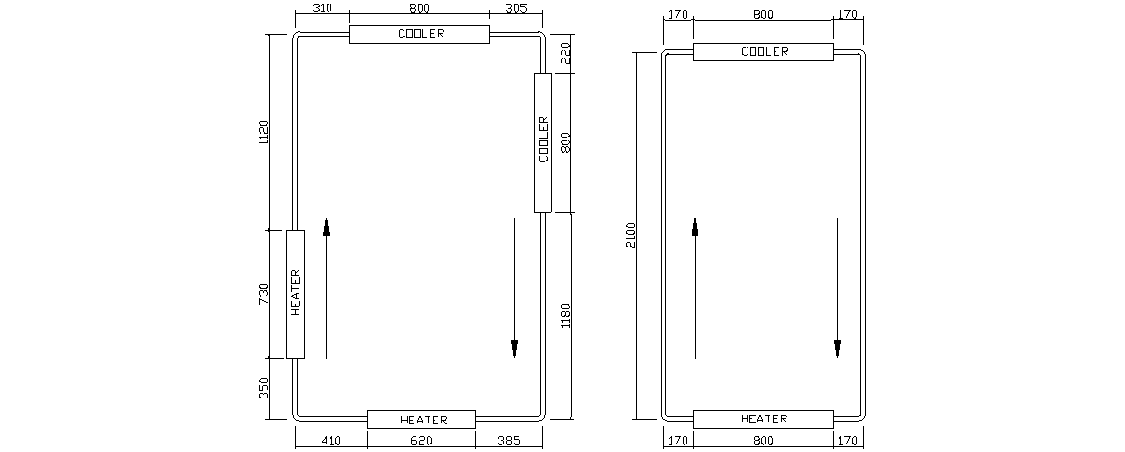
\includegraphics[width=\linewidth]{../imagens/pdf/LoopsBARC.pdf}
    \figcaption{Dimensões dos circuitos de convecção natural considerados para validação; à esquerda: circuito de \citet{VIJAYAN07}; à direita: circuito de \citet{VIJAYAN94}.}
    \label{fig_loopsbarc}
  \end{center}
\end{figure}

\begin{itemize}
  \item HHHC - aquecedor horizontal e arrefecedor horizontal;
  \item HHVC - aquecedor horizontal e arrefecedor vertical;
  \item VHHC - aquecedor vertical e arrefecedor horizontal;
  \item VHVC - aquecedor vertical e arrefecedor vertical.
\end{itemize}

A figura \ref{fig_validacao_perm} apresenta os resultados. Apesar de parecer um pouco confuso, o gráfico mostra boa aproximação obtida do modelo para o regime permanente. A tabela \ref{tab_validacao_perm} mostra resultados quantitativos da comparação, em termos do desvio médio\footnote{O desvio médio é a soma aritmética dos desvios relativos. Os desvios relativos foram computados para cada ponto como sendo o valor absoluto da diferença entre dado experimental $Re_{exp}$ e do modelo $Re_{mod}$ dividido pelo dado experimental, ou seja, $\text{desvio relativo} = |Re_{exp}-Re_{mod}|/Re_{exp}$.} e do coeficiente de determinação. O pior resultado é referente à configuração HHHC. Uma possível causa para o erro é a inexistência de informação quanto a perdas de carga locais.

\begin{figure}
  \begin{center}
    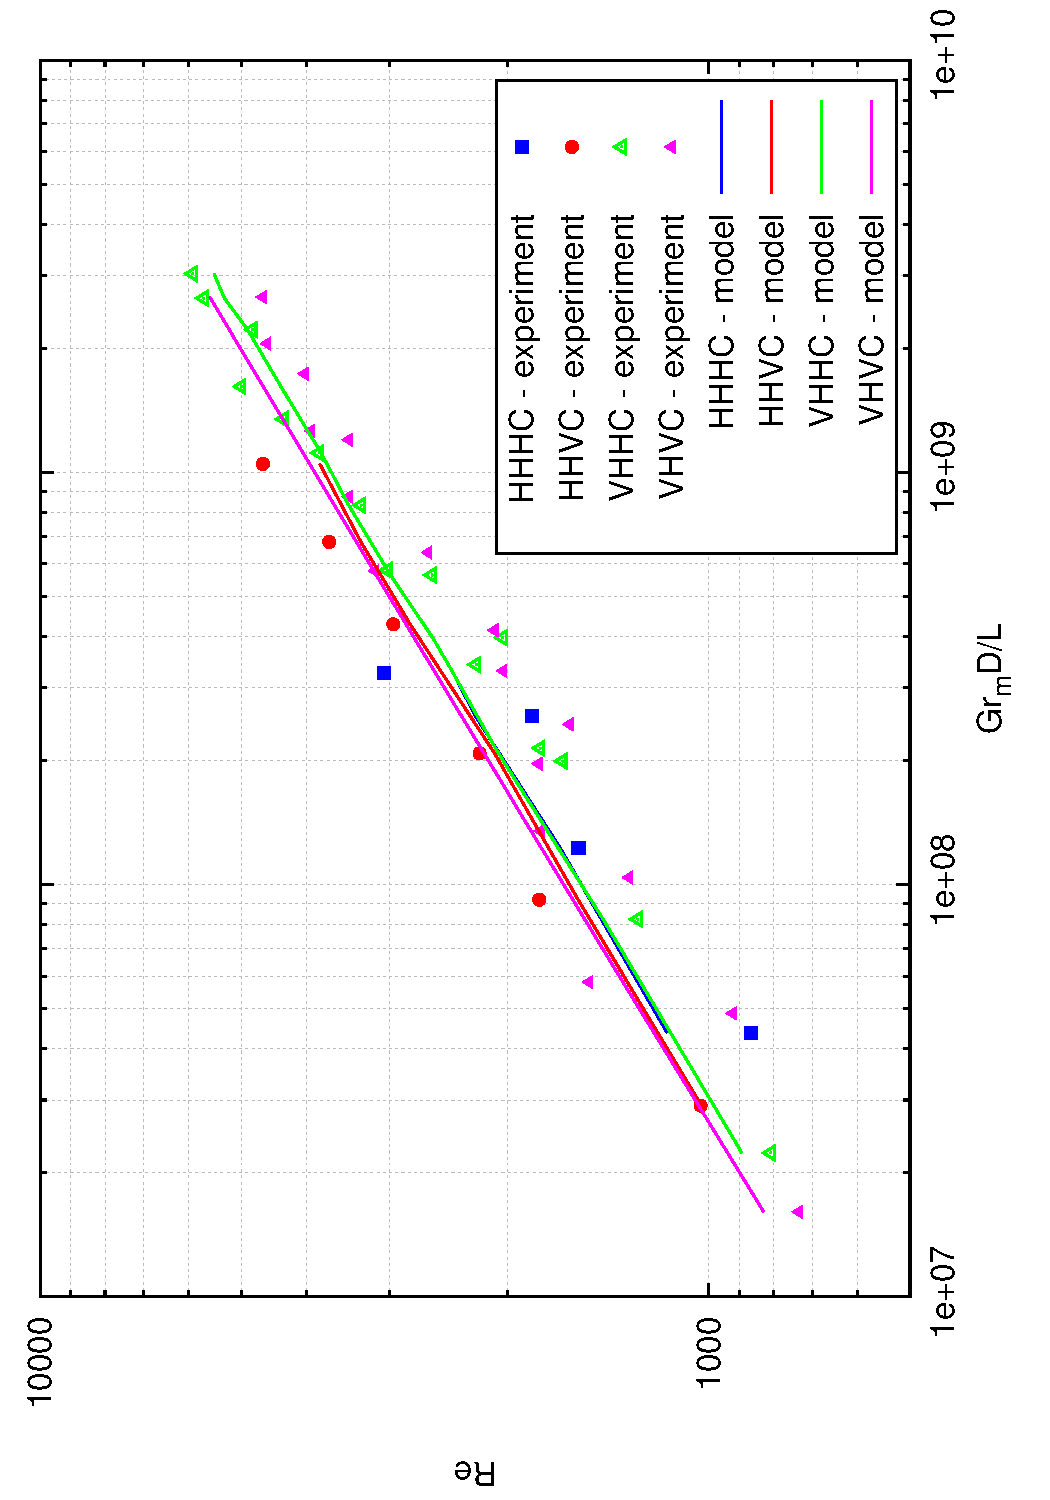
\includegraphics[width=.45\linewidth,angle=-90,origin=c]{../imagens/pdf/RexGrDL.pdf}
    \vspace*{-20mm}
    \figcaption{Comparação dos resultados fornecidos pelo modelo com dados experimentais publicados por \citet{VIJAYAN07} para todas as orientações de aquecedor e arrefecedor.}
    \label{fig_validacao_perm}
  \end{center}
\end{figure}

\begin{center}
  \begin{tabular}{ccccc}
    \hline
    & HHHC & HHVC & VHHC & VHVC\\
    \hline
    Desvio médio  & 20,67\% & 8,62\% & 10,30\% & 19,07\%\\
    Coeficiente de determinação & 0,60 & 0,87 & 0,94 & 0,89\\
    \hline\\
  \end{tabular}
  \tabcaption{Avaliação quantitativa dos resultados fornecidos pelo modelo em relação aos dados experimentais publicados.}
  \label{tab_validacao_perm}
\end{center}

\subsubsection{Validação para regime transiente}

A capacidade do modelo quanto à simulação de regimes transientes foi testada contra os dados experimentais de \citet{VIJAYAN94} e os resultados numéricos de \citet{AMBROSINI04}. 

\citet{VIJAYAN94} reportam o transiente da diferença de temperatura no aquecedor medida no experimento para o circuito de 23,2 mm de diâmetro. As mesmas condições do experimento foram simuladas pelo modelo, isto é, carga térmica de 420 W, coeficiente de troca de calor do arrefecedor igual a 1000 W/m$^2$/K, pressão de 1 bar e temperatura do fluido externo de 30ºC. Os parâmetros numéricos foram CFL = 0,4 e 800 pontos nodais, o que resultou num espaçamento de 8,1 mm entre nós de malha e passo de tempo de 0,0519 s. A condição inicial para o fluxo de massa foi de fluxo nulo e o campo de temperatura foi igual ao do regime permanente. O resultado da simulação é mostrado na figura \ref{fig_validacao_trans_01}. Os cálculos são interrompidos quando ocorre fluxo de massa negativo (o que indica reversão de fluxo).

A figura \ref{fig_validacao_trans_02} mostra a comparação com o experimento, excluindo as oscilações iniciais, indicando muito boa concordância. Em razão da limitação do código na ocorrência de reversão de fluxo, o a comparação pôde ser feita apenas para a faixa dos primeiros 80 s.

\begin{figure}[t]
  \begin{center}
    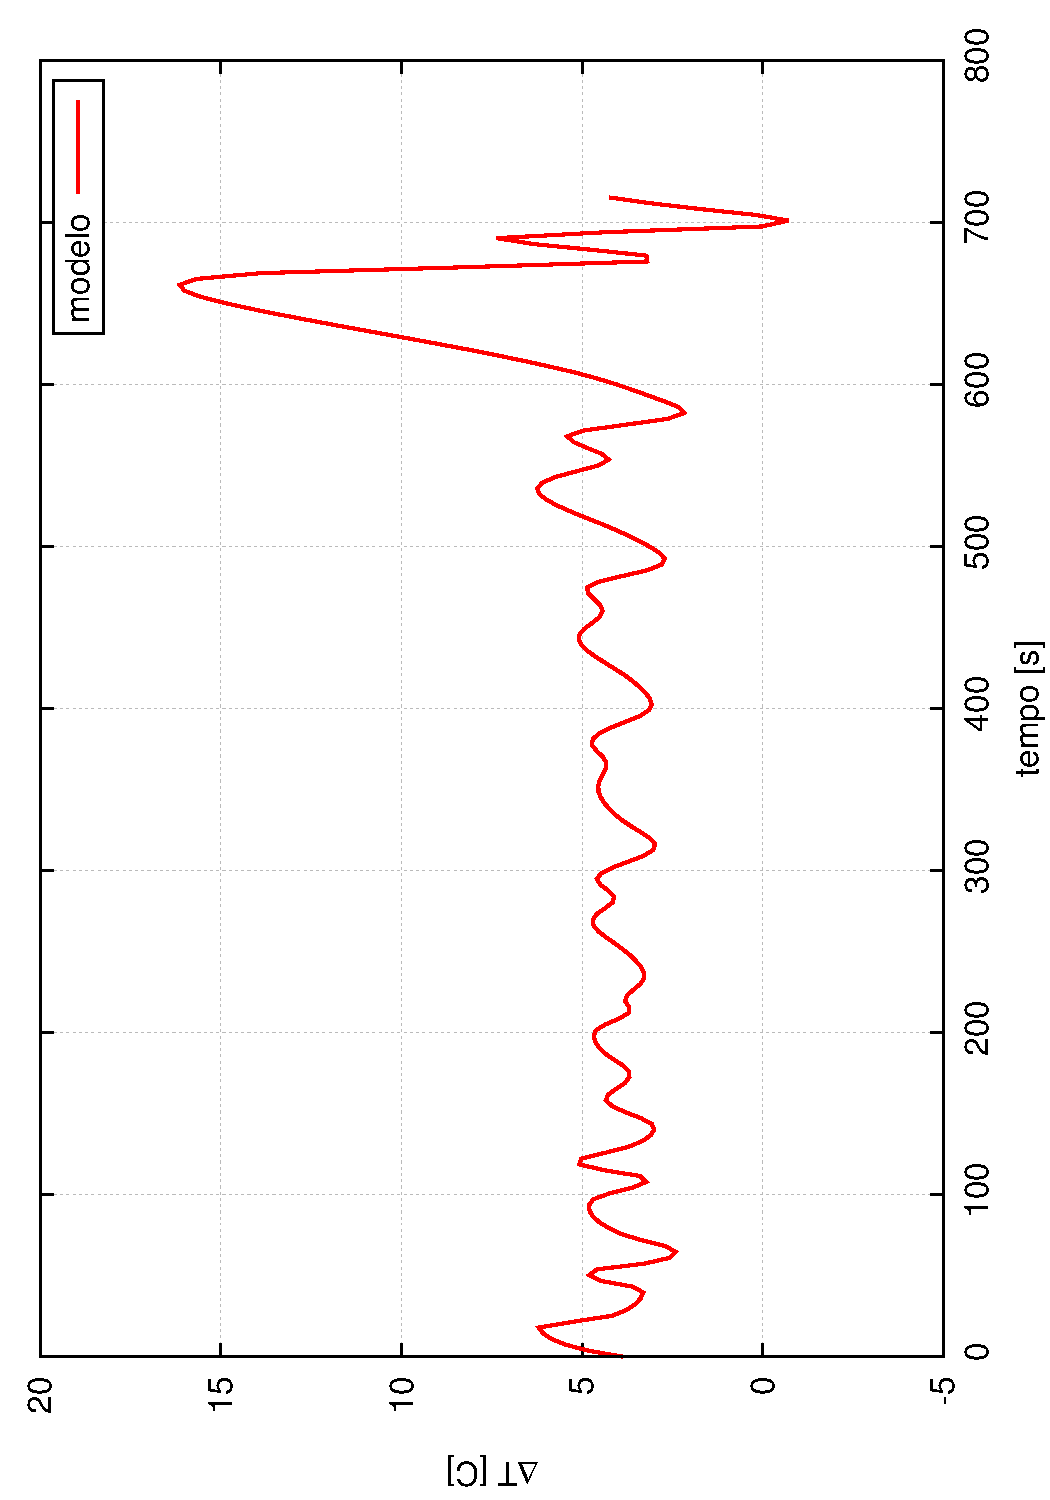
\includegraphics[width=.45\linewidth,angle=-90,origin=c]{../imagens/pdf/DT_heater_x_t_model_only.pdf}
    \vspace*{-15mm}
    \figcaption{Resultado do modelo para transiente da variação de temperatura no aquecedor, incluindo oscilações iniciais, para CFL=0,4.}
    \label{fig_validacao_trans_01}
  \end{center}
\end{figure}

\begin{figure}[t]
  \begin{center}
    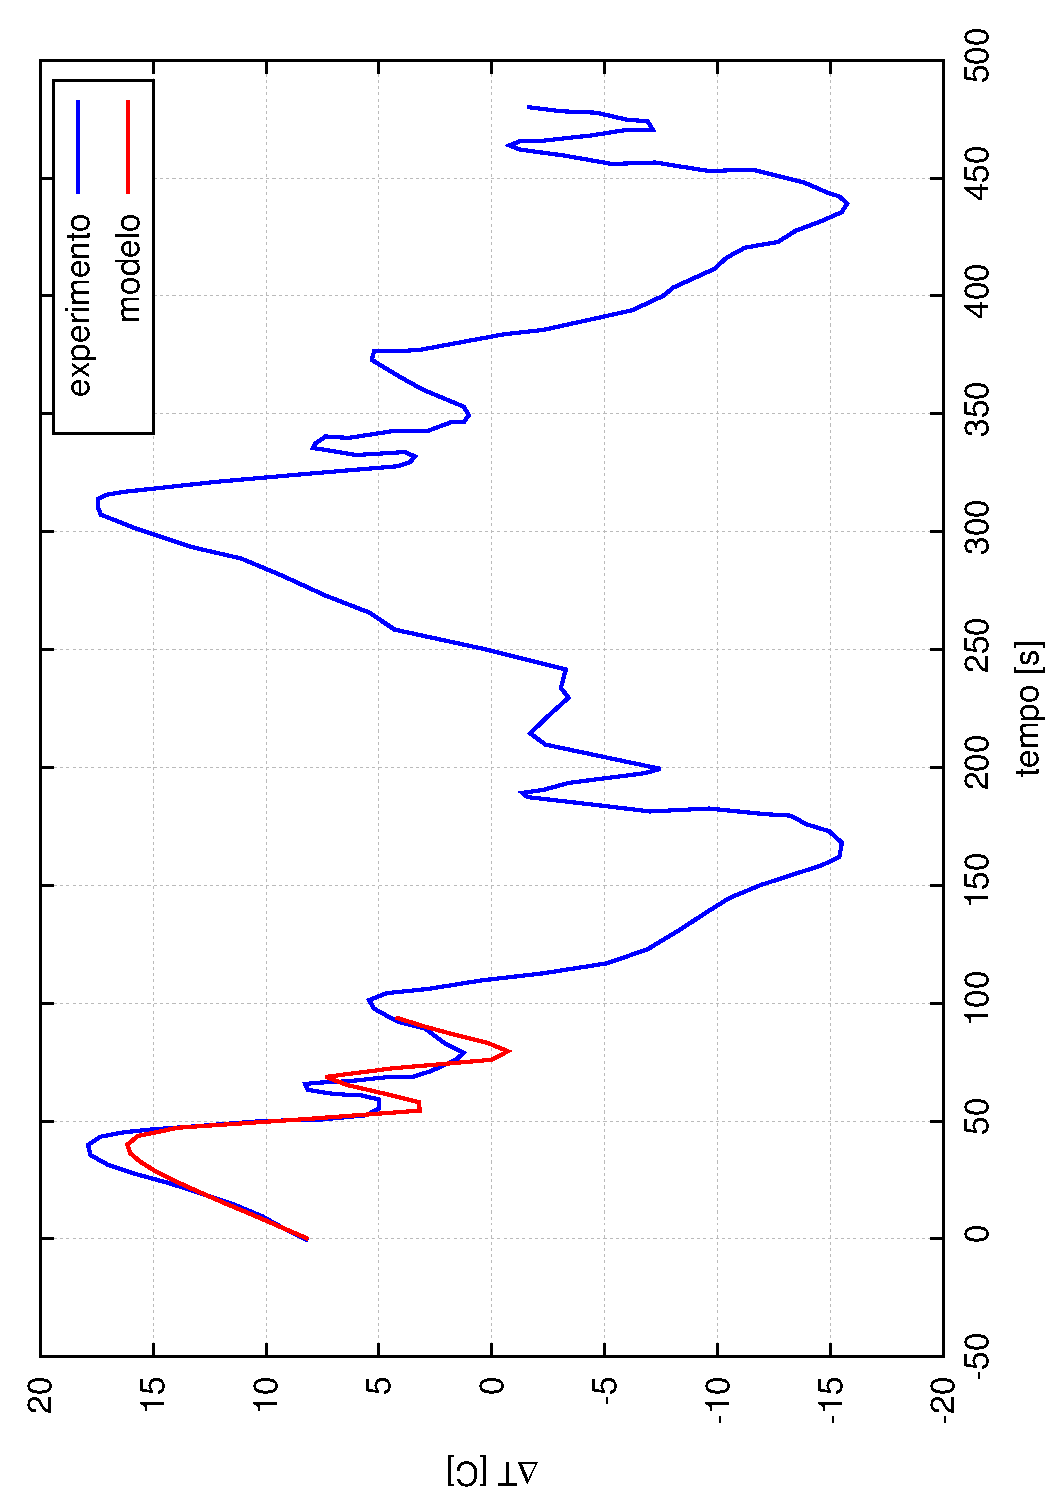
\includegraphics[width=.45\linewidth,angle=-90,origin=c]{../imagens/pdf/DT_heater_x_t.pdf}
    \vspace*{-15mm}
    \figcaption{Transiente da variação de temperatura no aquecedor: resposta do experimento de \citet{VIJAYAN95} e em comparação com o resultado obtido do modelo.}
    \label{fig_validacao_trans_02}
  \end{center}
\end{figure}

Um segundo teste, reduzindo CFL para 0,1, gerou resultado pior em relação ao experimento, antecipando a reversão do escoamento, conforme pode ser observado na figura \ref{fig_validacao_trans_03}. A conclusão preliminar é de que algumas perdas existentes no escoamento real são simuladas no modelo pela dissipação numérica, e que a redução do passo de tempo acaba resultando num escoamento menos dissipativo, o que aumenta a amplitude das oscilações e antecipa a reversão de fluxo. \citet{VIJAYAN95} empregaram o código computacional ATHLET para simular o experimento de \citet{VIJAYAN94}, e incluíram um modelo para a capacitância térmica das paredes, o que indica a relevância de mecanismos secundários de dissipação no escoamento.

O fator de atrito usado na geração desses resultados foi calculado como sendo o valor máximo entre as correlações de Poiseuille e Colebrook-White, conforme \citet{VIJAYAN95}. O fator de atrito segundo a correlação de Poiseuille é calculada em função do número de Reynolds por $f=16/Re$. A correlação de Colebrook-White implementada no modelo é implicitamente expressa por

\begin{equation}
  f^{-0,5} = -2\log_{10}\left(\frac{e}{3,7D} + \frac{2,51}{\Re f^{0,5}}\right)
\end{equation}
onde $f$ é o fator de atrito, $\Re$ é o número de Reynolds, $e$ é a rugosidade, para a qual foi utilizado o valor de $10^{-7}$, e $D$ é o diâmetro interno do circuito.

Em trabalho publicado em 2004, \citet{AMBROSINI04} estudaram o efeito do fator de atrito na modelagem de sistemas de convecção natural e concluíram que a escolha da correlação para atrito pode converter o escoamento simulado de estável para instável. Eles fizeram testes com as mesmas correlações usadas por \citet{VIJAYAN95} e compararam com a correlação de Churchill, dada por

\begin{eqnarray}
  f &=& 8\left[\left(\frac{8}{\Re}\right)^{12} + (A+B^{-1,5})\right]^{1/12}\\
  A &=& \left\{-2,457\ln\left[\left(\frac{7}{\Re}\right)^{0,9} + \frac{0,27e}{D}\right]\right\}^{16}\nonumber\\
  B &=& \left(\frac{37530}{\Re}\right)^{16}\nonumber
  \label{eq_churchill}
\end{eqnarray}

\begin{figure}
  \begin{center}
    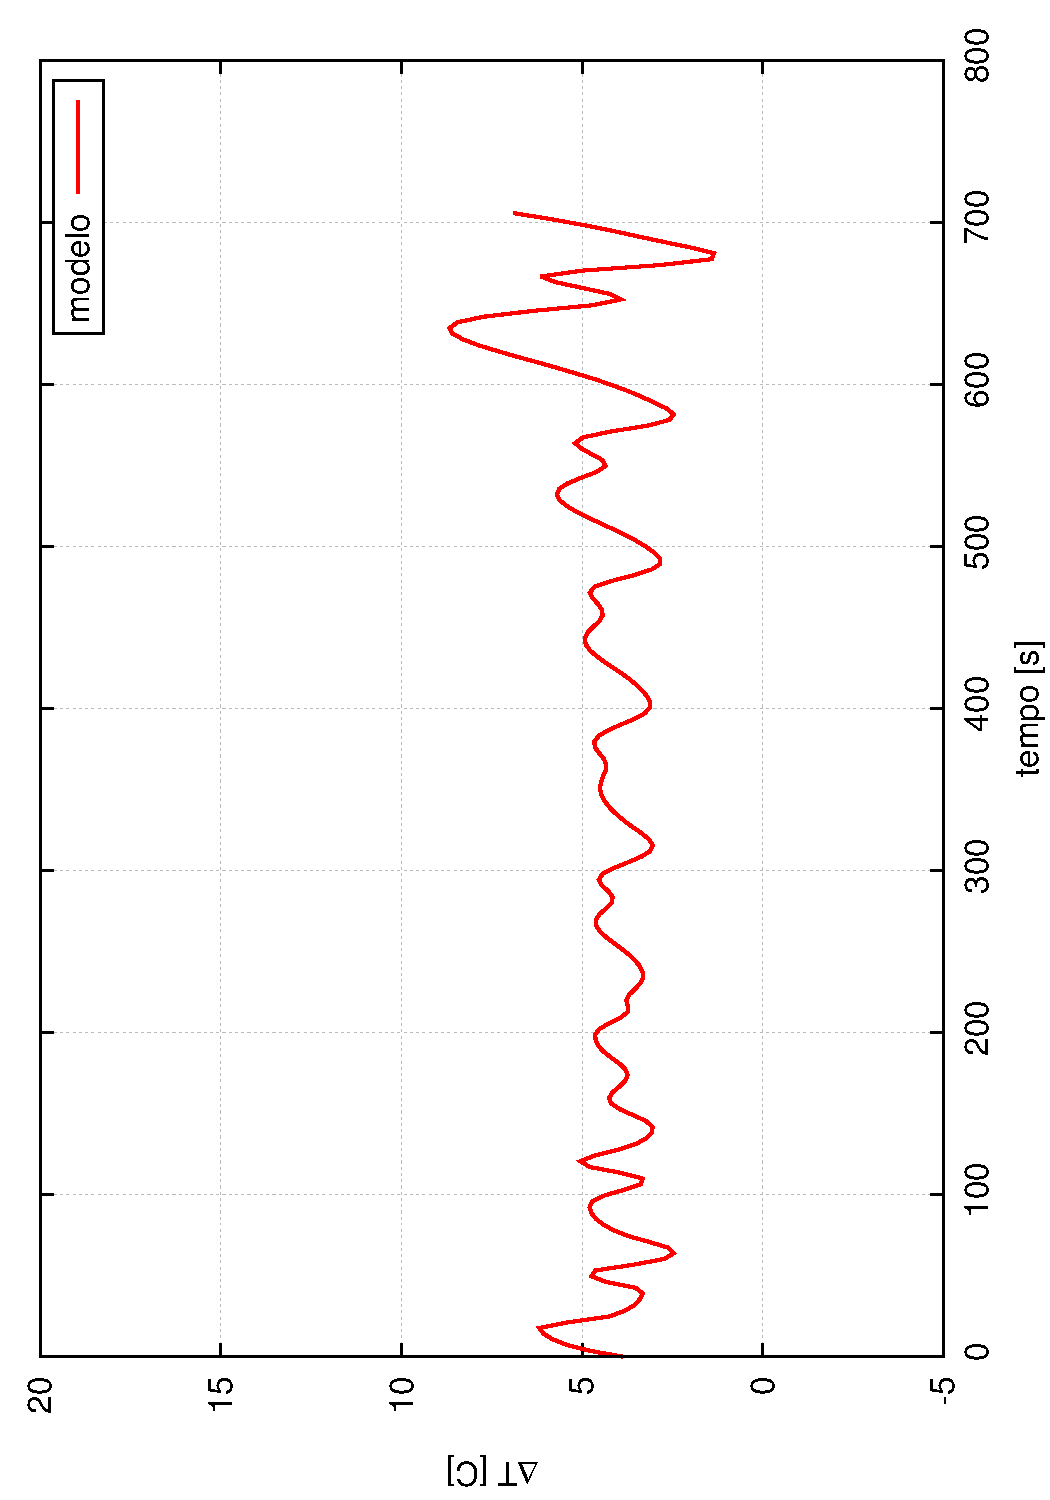
\includegraphics[width=.45\linewidth,angle=-90,origin=c]{../imagens/pdf/DT_heater_x_t_CFL01.pdf}
    \vspace*{-15mm}
    \figcaption{Resultado do modelo para transiente da variação de temperatura no aquecedor, incluindo oscilações iniciais, para CFL=0,1.}
    \label{fig_validacao_trans_03}
  \end{center}
\end{figure}

A correlação de Colebrook-White não é válida para todos os número de Reynolds, razão pela qual ela foi combinada com a expressão de Poiseuille. A correlação de Churchill é, em princípio, válida para todos os regimes de escoamento. \citet{AMBROSINI04} mostram mapas de estabilidade usando as duas formas de cálculo do fator de atrito, e concluem que o modelo que usa a correlação de Churchill gera uma região de estabilidade limitada a certas faixas de potência, enquanto que o modelo usando a combinação Poiseuille-Colebrook-White prediz instabilidade para toda a região testada.

Estes testes foram repetidos com o modelo aqui apresentado, mostrando resultados diferentes em relação aos encontrados por \citet{AMBROSINI04}. A tabela \ref{tab_limites_de_estabilidade} mostra os valores de potência que limitam a região de estabilidade segundo os cálculos de \citet{AMBROSINI04} e o presente modelo para temperatura do fluido externo igual a 30ºC, ambos usando a correlação de Churchill. \citet{AMBROSINI04} apresentam mais de um mapa de estabilidade usando a mesma correlação. Os valores mostrados na tabela a seguir são referentes aos resultados obtidos por eles para discretização de primeira ordem, usando método linear de análise de estabilidade (figura 8 do artigo deles).

\begin{center}
  \begin{tabular}{ccc}
    \hline
    & limite inferior & limite superior\\
    \hline
    \citet{AMBROSINI04} & 285 W & 480 W\\
    presente modelo & 390 W & 707 W\\
    \hline\\
  \end{tabular}
  \tabcaption{Limites de estabilidade usando a correlação de Churchill para o fator de atrito, com temperatura do fluido externo igual a 30ºC.}
  \label{tab_limites_de_estabilidade}
\end{center}

A explicação dada por \citet{AMBROSINI04} para a ocorrência de uma região de estabilidade usando a correlação de Churchill se baseia no vale gerado na curva do fator de atrito em função do número Reynolds na região de transição entre o regime laminar e o turbulento. A conclusão após essa comparação é que o presente modelo fornece os mesmos resultados de \citet{AMBROSINI04} do ponto de vista qualitativo, mas a faixa de estabilidade é deslocada para regiões de potências mais altas.

Com a correlação de Poiseuille-Colebrook-White, \citet{AMBROSINI04} não encontraram região de estabilidade, enquanto que o presente modelo previu escoamentos estáveis para potências abaixo de 235 W. %Uma possível resposta para esse comportamento é que os valores do fator de atrito para a região de transição entre regimes laminar e turbulento segundo esta correlação são mais altos em relação à fórmula de Churchill, tendendo a estabilizar o escoamento nessa região.

A razão para a discrepância entre as resultados do presente modelo e \citet{AMBROSINI04} ainda é desconhecida. Eles, por exemplo, afirmam que o número de Reynolds para regime permanente nas mesmas condições é de aproximadamente 2700, enquanto que este modelo fornece $\Re = 2377$ com a correlação de Churchill e $\Re = 2180$ com Poiseuille-Colebrook-White, resultados que devem ser julgados como resultados confiáveis depois da validação com relação ao regime permanente.

%\subsubsection{Análises de estabilidade}

\section{Sistema Passivo de Resfriamento da UFC}

A Unidade de Armazenamento Complementar de Elementos Combustíveis Irradiados -- UFC -- é uma instalação nuclear que está sendo projetada pela \href{www.eletronuclear.gov.br}{Eletrobras Eletronuclear} e terão a finalidade de armazenar os elementos combustíveis irradiados (ECIs) nas unidades da Central Nuclear Almirante Álvaro Alberto, no município de Angra dos Reis. Os ECIs serão acomodados num tanque preenchido com água desmineralizada, que absorverá o calor de decaimento rejeitado por eles. Para transferir esse calor para uma fonte fria final, a Unidade UFC contará com um sistema de remoção de calor, que operará unicamente por convecção natural. 

Segundo o projeto conceitual da Unidade, o sistema de remoção de calor será um SPR monofásico, operando com água, e deverá transferir 2800 kW quando a capacidade total de armezamento estiver ocupada. A fonte fria final será o ar ambiente externo. Segundo a base normativa adotada para projeto do sistema, três condições operacionais devem ser consideradas no dimensionamento do sistema: condição normal, condição anormal e acidente. A cada um desses cenários está associado um limite para a temperatura da água do tanque de armazenamento e outro para a temperatura do ar externo. O sistema de remoção de calor será modular, e a quantidade postulada de módulos disponíveis também varia conforme a condição de operação. A tabela \ref{tab_condicoes_de_operacao} resume as temperaturas e capacidades de projeto do sistema de remoção de calor em função da condição de operação.

\begin{center}
\begin{tabular}{cccc}
  \hline
  condição de operação & limite temperatura tanque & temperatura fonte fria & capacidade do sistema\\
  \hline
  normal   & 45 ºC & 28,3 ºC & 17,50 kW / módulo\\
  anormal  & 60 ºC & 33,0 ºC & 21,87 kW / módulo\\
  acidente & 80 ºC & 33,0 ºC & 43,75 kW / módulo\\
  \hline\\
\end{tabular}
  \tabcaption{Limite de temperatura no tanque, temperatura da fonte fria e capacidade do sistema de remoção de calor em função da condição de operação. A capacidade do sistema é apresentada através da carga térmica máxima (2800 kW) dividida pelo número postulado de módulos disponíveis.}
\label{tab_condicoes_de_operacao}
\end{center}

Estudos experimentais de viabilidade do sistema foram realizados na Universidade Técnica de Dresden. O aparato de teste consistiu de um trocador de calor água-água, imerso num tanque que recebia uma carga térmica controlada. Os trocadores água-água eram conectados por uma tubulação a trocadores de calor água-ar instalados numa torre seca de resfriamento. O modelo desenvolvido neste trabalho foi utilizado para simular este aparato de teste, com a finalidade de verificar a aplicabilidade do modelo a um sistema com características geométricas mais complexas. Para tanto, o sistema de teste real foi simplificado no modelo para um {\it loop} com as características dos {\it loops} experimentais da figura \ref{fig_loopsbarc}, resultando nos seguintes parâmetros:

\begin{itemize}
\item diâmetro interno: 60 mm;
\item largura: 20 m;
\item altura: 5,8 m;
\item distância entre linhas de centro dos trocadores: 4 m;
\item perdas de carga totais no circuito: 30.
\end{itemize}

Dados estacionário experimentais obtidos do aparato de teste relacionando o carga térmica fornecida ao sistema com a diferença de temperatura entre fonte quente e fonte fria foram adotados como referência. A tabela \ref{tab_modelo_x_luka} lista as condições de referência e os resultados fornecidos pelo modelo, apresentando as temperaturas de entrada e saída do aquecedor e a vazão.

\begin{center}
\begin{tabular}{ccccc}
  \hline
  carga térmica & dif. temp. exp. & temp. entrada aquec. modelo & temp. saída aquec. modelo & vazão\\
  \hline
  10 kW & 18,2 ºC & 46,5 ºC & 35,6 ºC & 0,23 kg/s\\
  15 kW & 24,3 ºC & 53,9 ºC & 40,1 ºC & 0,28 kg/s\\
  20 kW & 30,0 ºC & 61,0 ºC & 44,8 ºC & 0,32 kg/s\\
  \hline\\
\end{tabular}
  \tabcaption{Verificação da capacidade do modelo na simulação de um SPR com geometria complexa. As duas primeiras colunas à esquerda são dados experimentais e as três demais colunas são resultados fornecidos pelo modelo.}
\label{tab_modelo_x_luka}
\end{center}

Foi observado no aparato de teste que as perdas calor na tubulação do circuito são muito pequenas, e podem ser desprezadas. Também foi observado que a diferença entre a temperatura de saída do aquecedor e a do tanque varia entre 1 ºC e 2 ºC, e que a diferença entre a temperatura de entrada no aquecedor e a de saída do ar no arrefecedor varia entre 6 ºC e 15 ºC. Assumindo, portanto, um acréscimo de 10 ºC na diferença de temperatura entre saída e entrada do aquecedor nos resultados do modelo, é possível concluir que os dados fornecidos pelo modelo concordam qualitativamente com os do experimento. A vazão mássica no circuito prevista pelo modelo também está na faixa das vazões medidas no experimento. A correlação de Churchill (equação \ref{eq_churchill}) foi utilizada para o cálculo do fator de atrito.

Após esta verificação, o modelo foi aplicado na simulação das condições normais de operação do Sistema de Remoção de Calor da Unidade UFC, utilizando os seguintes parâmetros:

\begin{itemize}
\item pressão no circuito: 1 bar;
\item carga térmica: 17,5 kW;
\item temperatura da fonte fria: 28,3 ºC
\end{itemize}

Essas condições foram simuladas com as características geométricas do aparato de teste, as quais incluem uma diferença de 3,8 m entre as alturas médias dos trocadores de calor. Em seguida, as mesmas condições operacionais foram simuladas, porém aumentando essa diferença de alturas para 20. Os resultados são sumarizados na tabela \ref{tab_modelo_x_UFC}.

\begin{center}
\begin{tabular}{ccccc}
  \hline
  carga térmica & dif. alturas & temp. entrada aquec. modelo & temp. saída aquec. modelo & vazão\\
  \hline
  17,5 kW & 3,8 m & 56,7 ºC & 41,3 ºC & 0,29 kg/s\\
  17,5 kW & 20,0 m & 53,7 ºC & 43,4 ºC & 0,48 kg/s\\
  \hline\\
\end{tabular}
  \tabcaption{Simulação do Sistema de Remoção de Calor segundo o modelo desenvolvido para duas diferenças de altura diferentes.}
\label{tab_modelo_x_UFC}
\end{center}

Os resultados mostram que o aumento da diferença de altura entre os trocadores não produz uma redução significativa na temperatura máxima do circuito e, consequentemente, no tanque. A maior altura do circuito aumentou em 65 \% a vazão, mas a temperatura média no circuito permaneceu a mesma. 

Estes resultados, apesar de carecerem de uma maior precisão nos parâmetros de entrada, são uma indicação de que um aumento na altura do circuito pode não fornecer a capacidade de remoção desejada.

Por último, cabe afirmar que os regimes transientes em todas as condições mostraram comportamentos estáveis.

\singlespacing

\bibliographystyle{plainnat}
\bibliography{../../referencias/ref}

%\end{multicols}
\end{document}
